\section{Ejercicio 3: Amplificador de instrumentaci\'on} 
\subsection{Introducci\'on}
\paragraph{Amplificador diferencial}
Un amplificador diferencial es un dispositivo que amplifica la $\textit{diferencia}$ de las se\~nales en sus entradas. El principio de funcionamiento de este amplificador es la de, asumiendo que el ruido introducido en sus entradas es igual para todas ellas,  la diferencia entre las se\~nales comunes, en modo com\'un(el ruido por ejemplo), es nula, por lo tanto es atenuada infinitamente. Se obtiene a la salida la amplificaci\'on de las se\~nales en modo diferencial.
Se muestra en la Figura \ref{fig:AMP_DIF}  el amplificador diferencial con un modelo de las entradas en modo com\'un y modo diferencial.
\begin{figure}[H]

    \centering
    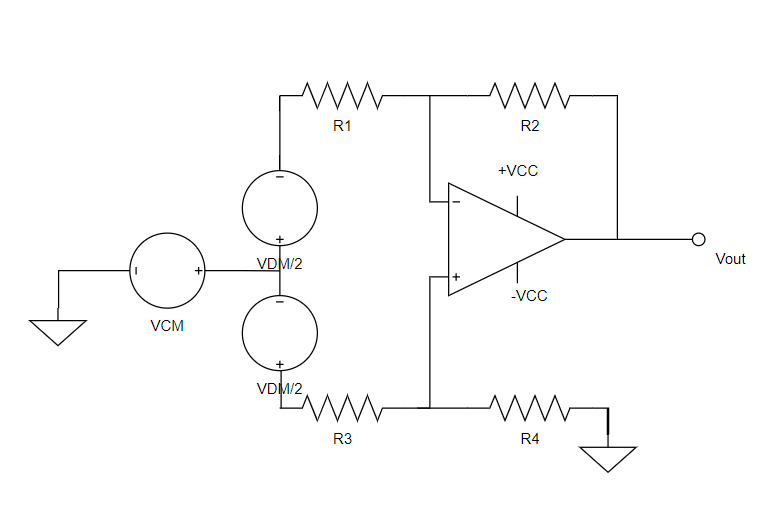
\includegraphics[width=0.5\textwidth]{../EJ3/Recursos/AMP_DIF}
    \caption{Amplificador diferencial b\'asico}
    \label{fig:AMP_DIF}
\end{figure}

En la realidad no se consigue el funcionamiento ideal descripto anteriormente, luego es necesario introducir los conceptos de $A_{DM}$, $A_{CM}$ y $CMRR$. $A_{DM}$ indica la ganancia en modo diferencial del circuito, $A_{CM}$ indica la ganancia en modo com\'un y $CMRR$ o Common Mode Rejection Ratio indica la relaci\'on entre ambas, lo que muestra cuantitativamente cuanto rechaza el circuito, se\~nales en modo com\'un. Este se calculado como se muestra en \ref{eq:CMRR}

 \begin{equation}
    CMRR=20 \cdot \log \left| \frac{A_{DM}}{A_{CM}} \right|
    \label{eq:CMRR}
 \end{equation}
\paragraph{Amplificador de instrumentaci\'on}
El amplificador de instrumentaci\'on es un amplificador diferencial de precisi\'on que parte de los conceptos explicados anteriormente. Sin embargo se introduce a su entrada una etapa sim\'etrica previa, con entrada y salida diferencial, que aumenta la impedancia de entrada y permite dividir la ganancia en dos etapas. Las caracter\'isticas pricipales de este circuito son su alta impedancia de entrada, una baja impedancia de salida y un alto $CMRR$.

\subsection{An\'alisis te\'orico}
Se presenta en la Figura \ref{fig:AMP_INST} el amplificador de instrumentaci\'on analizado en esta secci\'on.
\begin{figure}[H]

    \centering
    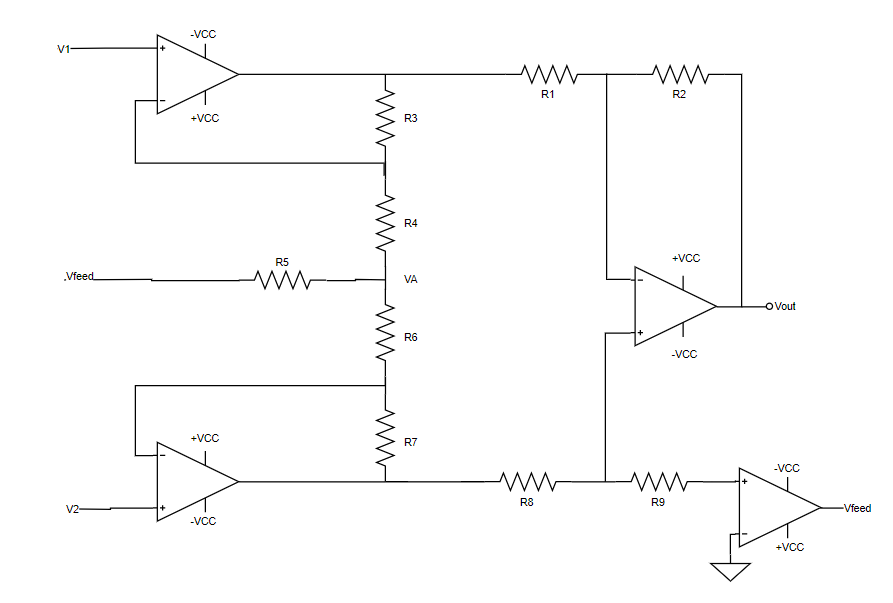
\includegraphics[width=0.5\textwidth]{../EJ3/Recursos/AMP_INST}
    \caption{Amplificador de instrumentaci\'on utilizado}
    \label{fig:AMP_INST}
\end{figure}
Si se compara el circuito de la figura, con la configuraci\'on de amplificador de instrumentaci\'on descripta anteriormente, se observa que se agrega el amplificador operacional $U4$. La funci\'on de este \'ultimo es la de fijar un potencial cercano a los $0V$ en el nodo $VA$, conservando la simetria. Esto es de suma importancia porque, con esta condici\'on y aplicando el Teorema de Bartlett con el modelo de modo com\'un, es posible analizar el circuito como se muestra en la Figura \ref{fig:SIMETRICO} 
\begin{figure}[H]

    \centering
    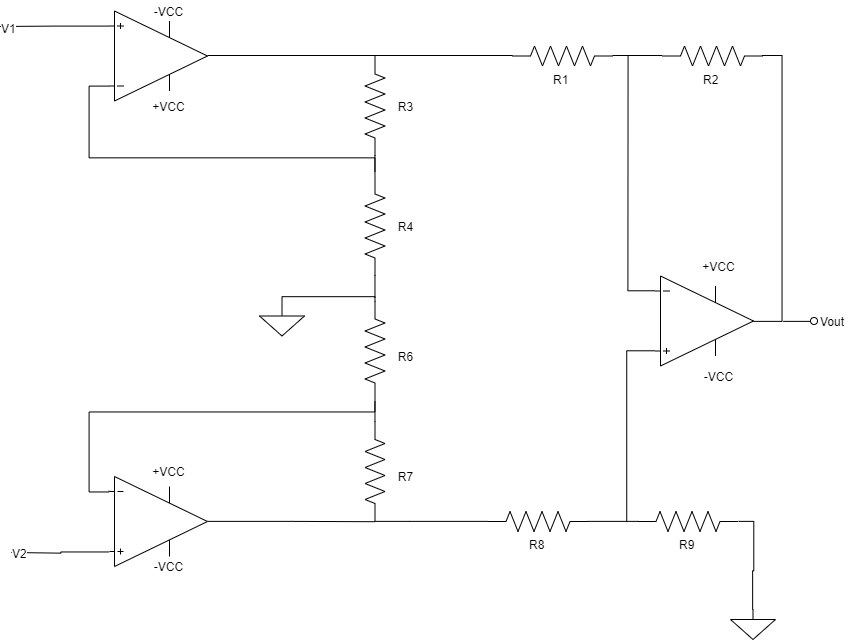
\includegraphics[width=0.5\textwidth]{../EJ3/Recursos/SIMETRICO}
    \caption{Circuito equivalente con realimentaci\'on, para modo com\'un}
    \label{fig:SIMETRICO}
\end{figure}
Se puede ver entonces que, trabajando en modo com\'un, la etapa de la entrada amplifica igual en ambas entradas y luego es atenuado por la etapa restadora.
\subsubsection{Asumiendo amplificadores operacionales ideales}
Se presenta en \ref{eq:sist_ideal} el sistema de ecuaciones del que se parte para obtener la respuesta del sistema.
\begin{equation}
        \left\{
            \begin{array}{llll}
                
                V_{o2} = 0 &\\
                
                V_{o1} = V_{1}\cdot \left(1+\frac{R_3}{R_4}\right) - V_A\cdot\frac{R_3}{R_4}\\
                
                V_A = V_2\cdot \left(1+\frac{R_6}{R_7}\right)\\
                
                V_{out} = \left(1+\frac{R_2}{R_1}\right)\cdot V_{o2} -  \frac{R_2}{R_1} \cdot V_{o1}
            \end{array}
        \right.
  \label{eq:sist_ideal}
\end{equation}
Se obtiene de ese sistema entonces la tensi\'on de salida $V_{out}$ en funci\'on de $V_1 $ y $V_2$ que se muestra en \ref{eq:soluc_ideal}
\begin{equation}
    V_{out} =  -  \frac{R_2}{R_1} \cdot \left(V_{1}\cdot \left(1+\frac{R_3}{R_4}\right) - V_2\cdot \left(1+\frac{R_6}{R_7}\right)\cdot\frac{R_3}{R_4}\\\right)
    \label{eq:soluc_ideal}
\end{equation}
Luego, para que la atenuaci\'on del modo com\'un  sea m\'axima y el $CMRR$ sea infinito, se impone la condici\'on $V_1 = V_2 \implies V_{out} = 0V$. Partiendo de \ref{eq:soluc_ideal} e imponiendo esta condici\'on se llega a la condici\'on de puente balanceado, que se muestra en \ref{eq:puente_balanceado}, para las resistencias de la etapa de entrada del amplificador.
\begin{equation}
    R_7\cdot R_4 = R_6 * R_3
    \label{eq:puente_balanceado}
\end{equation}
Finalmente se obtiene \ref{eq:soluc_final} que se utiliza, en conjunto con \ref{eq:puente_balanceado}, para elegir algunos de los valores de resistencias a utilizar.
\begin{equation}
    V_{out} = -\frac{R_2}{R_1} \cdot \left(1+\frac{R_3}{R_4}\right)\cdot \left(V_1-V_2\right)
    \label{eq:soluc_final}
\end{equation}
\subsubsection{Amplificadores operacionales no ideales }
En esta secci\'on se hace el an\'alisis del circuito en el caso de $A_{vol}$ finito con polo dominante. Adem\'as se asume que todos los operacionales tiene igual $A_{vol}$.

Utilizando el m\'etodo de resoluci\'on por nodos se obtiene el sistema de 9 ecuaciones \ref{eq:sistema_9}.
\begin{equation}
    \left\{
        \begin{array}{lllllllll}
            
            V_{o1} = (V_1-V_1^-)\cdot A_{vol} &\\
            
            V_{o2} = (V_2-V_2^-)\cdot A_{vol}\\
            
            V_{out} = (V_{o2}-V_3^-)\cdot A_{vol}\\
            
            V_{feed} = V_{o2}\cdot A_{vol}\\

            \frac{V_{o1}-V_1^-}{R_3} = \frac{V_1^- - V_A}{R_4}\\

            \frac{V_{A}-V_2^-}{R_6} = \frac{V_2^- - V_{o2}}{R_7}\\

            \frac{V_{o1}-V_3^-}{R_1} = \frac{V_3^- - V_{out}}{R_2}\\

            \frac{V_{feed}-V_A}{R_5} + \frac{V_1^- - V_A}{R_4}= \frac{V_A - V_2^-}{R_6}\\

            A_{vol} = \frac{A_o}{1+\frac{s}{\omega_p}}
        \end{array}
    \right.
\label{eq:sistema_9}
\end{equation}
Debido a la complejidad que representa este sistema, se recurre para resolverlo a un software de matem\'atica.
Sin embargo la soluci\'on es tan extensa que no tiene sentido incluirla, debido a que no se pueden obtener conclusiones a partir de ella.
Adem\'as, se puede observar que, modificando convenientemente los $A_o$ de cada uno de los operacionales, es posible realizar un an\'alisis en el que algunos operacionales tienen comportamiento ideal y otros no. 


\subsection{Dise\~no, simulaciones y mediciones}
En esta secci\'on se describen las caracter\'isticas constructivas a utilizadas en el circuito.

\subsubsection{Elecci\'on de componentes}
En base a \ref{eq:puente_balanceado} y \ref{eq:soluc_final} se realiza la selecci\'on de los componentes, obteni\'endose los valores que se muestran en \ref{eq:valores_deR}, \'unicamente en base a la ganancia que se desea obtener en modo diferencial, de 130 veces.
\begin{equation}
    \begin{array}{llll}
        R_1 = 6.8 K\Omega\\
        R_2 = 68 K\Omega\\
        R_4 = R_6 = 1.5 K\Omega\\
        R_3 = R_7 = 18 K\Omega \\
    \end{array}
\label{eq:valores_deR}    
\end{equation}
Debido a que peque\~nas variaciones en los componentes afectan la simetr\'ia del circuito, que es lo que permite que el CMRR sea muy alto, se decide utilizar resistencias SMD y de tolerancia de 1\%. 
En principio, no hay l\'imites es cuanto a los valores de estas resistencias, \'unicamente una relaci\'on, sin embargo se utilizan valores de resistencia medios. Si estos fueran muy altos, aumenta el nivel de ruido introducido al circuito por las resistencias, que como se sabe es mayor a medida que aumenta el valor de resistencia y es proporcional a $\sqrt{R}$

Para $R_8$ y $R_9$, de los cuales en ning\'un caso se obtuvo ning\'un par\'ametro en las ecuaciones, se recurre a las simulaciones relizadas, donde se observa que se obtiene el mejor resultado posible en t\'erminos de rechazo al modo com\'un y ganancia.

Para $R_5$, si bien se vieron variaciones en el an\'alisis te\'orico no son lo suficientemente significativos como para tomar una decisi\'on acerca de un valor. Nuevamente se recurre a las simulaciones, y se observa que para valores muy bajos de $R_5$, menores a $10 K\Omega$ el circuito se vuelve inestable y oscila, y para valores mayores a $100 K\Omega$ baja el CMRR, en particular para frecuencias mayores a 10KHz. Por estas razones se decide utilizar,en el PCB, un preset de $50 K\Omega$ y adem\'as una resistencia fija de $30 K\Omega$, un valor intermedio y que permite que el circuito se comporte de manera esperada. 

Finalmente, para el amplificador operacional, se decide utilizar el TL084. Esto debido a sus caracter\'isticas, como impedancia de entrada, $A_o$ y GPB, que lo hacen acercarse al modelo ideal del amplificador operacional. Con este comportamiento es posible elevar el CMRR. 

\subsubsection{Curvas obtenidas a partir an\'alisis te\'orico }
En esta secci\'on se presentan las curvas obtenidas a partir del an\'alisis te\'orico realizado anteriormente, con los valores de resistencia elegidos. Adem\'as se repite el an\'alsis para distintos casos de configuraciones de algunos operacionales reales y otros ideales. Las configuraciones comparadas son U1 y U2 ideales, U3 y U4 ideales y, por \'ultimo, ninguno de los amplificadores operacionales ideal. 
En la Figura \ref{fig:Comp_diff} se puede observar la comparaci\'on de modulo y fase de la transferencia en modo diferencial, y en la Figura \ref{fig:Comp_common} el mismo an\'alisis pero para modo com\'un.
Para los datos que son dependientes del amplificador operacional, como $A_o$ y $\omega_p$ (en realidad de utiliza GBP) se utilizaron los datos de la \href{https://www.egr.msu.edu/eceshop/Parts_Inventory/datasheets/tl084cn.pdf}{hoja de datos del TL084}. 

\begin{figure}[H]
    \centering
\resizebox{\textwidth}{!}{%
\begin{tabular}{c c}
    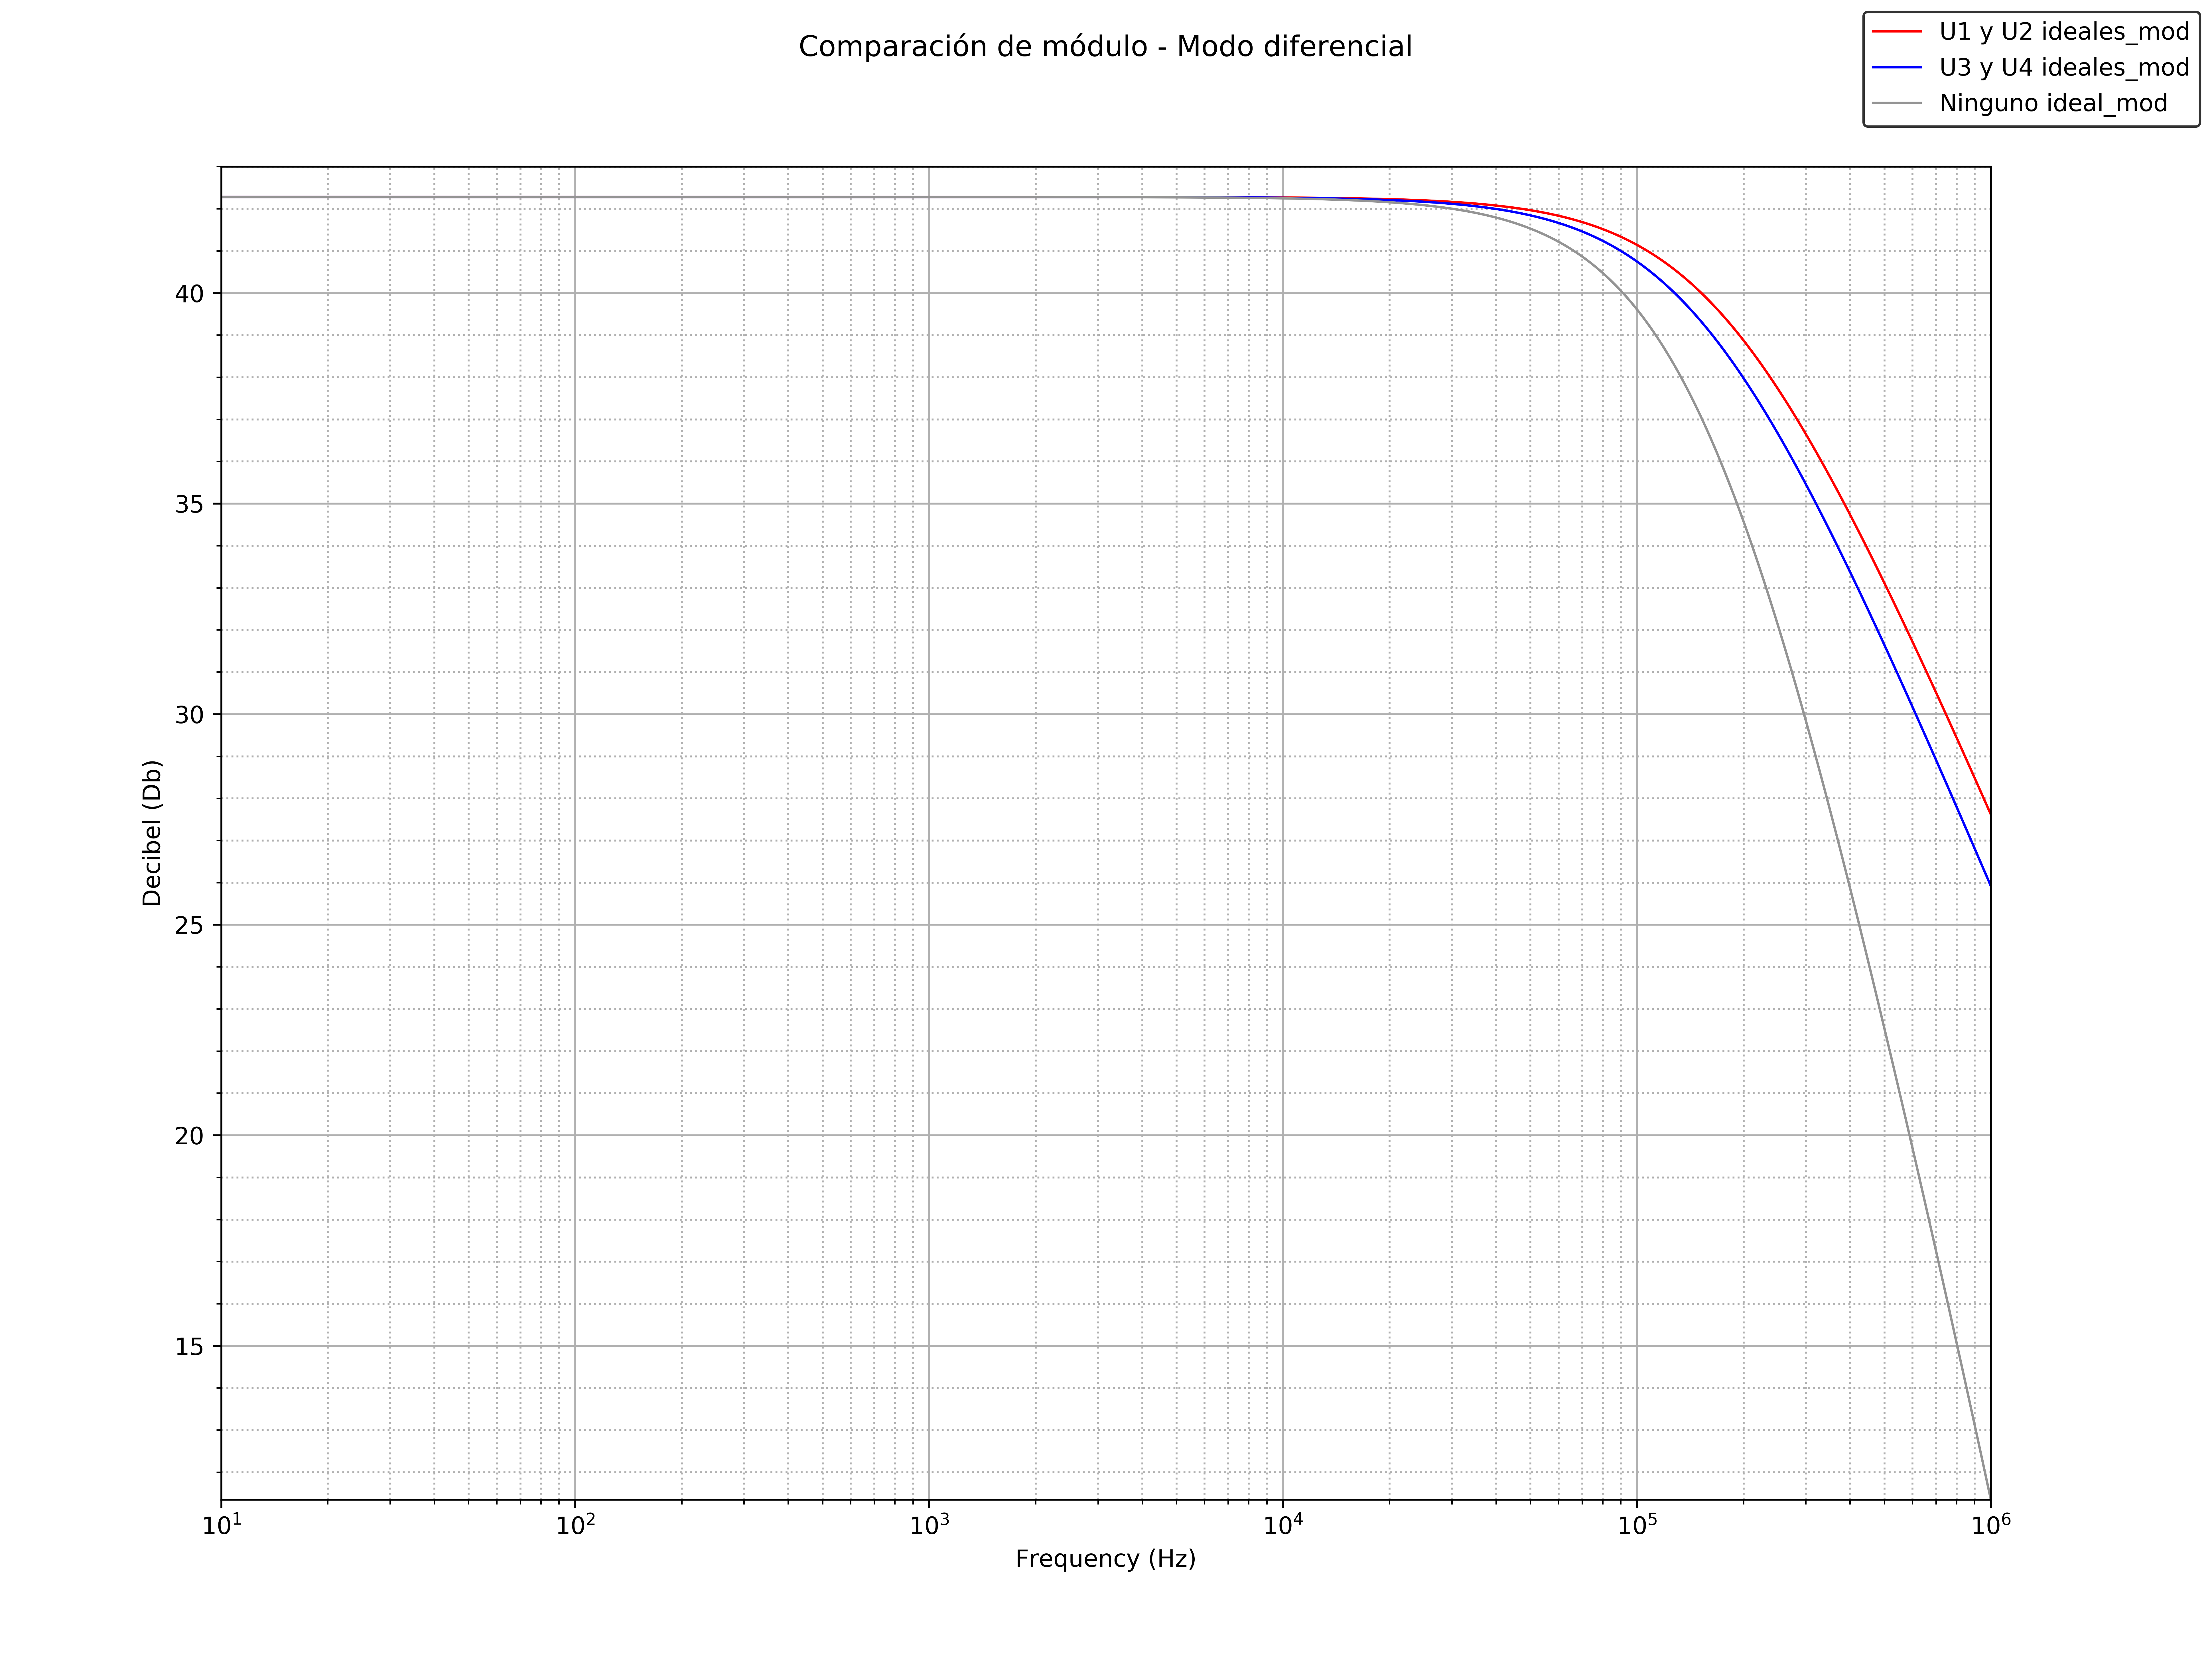
\includegraphics{../EJ3/Recursos/Comp_mod_diff} &
    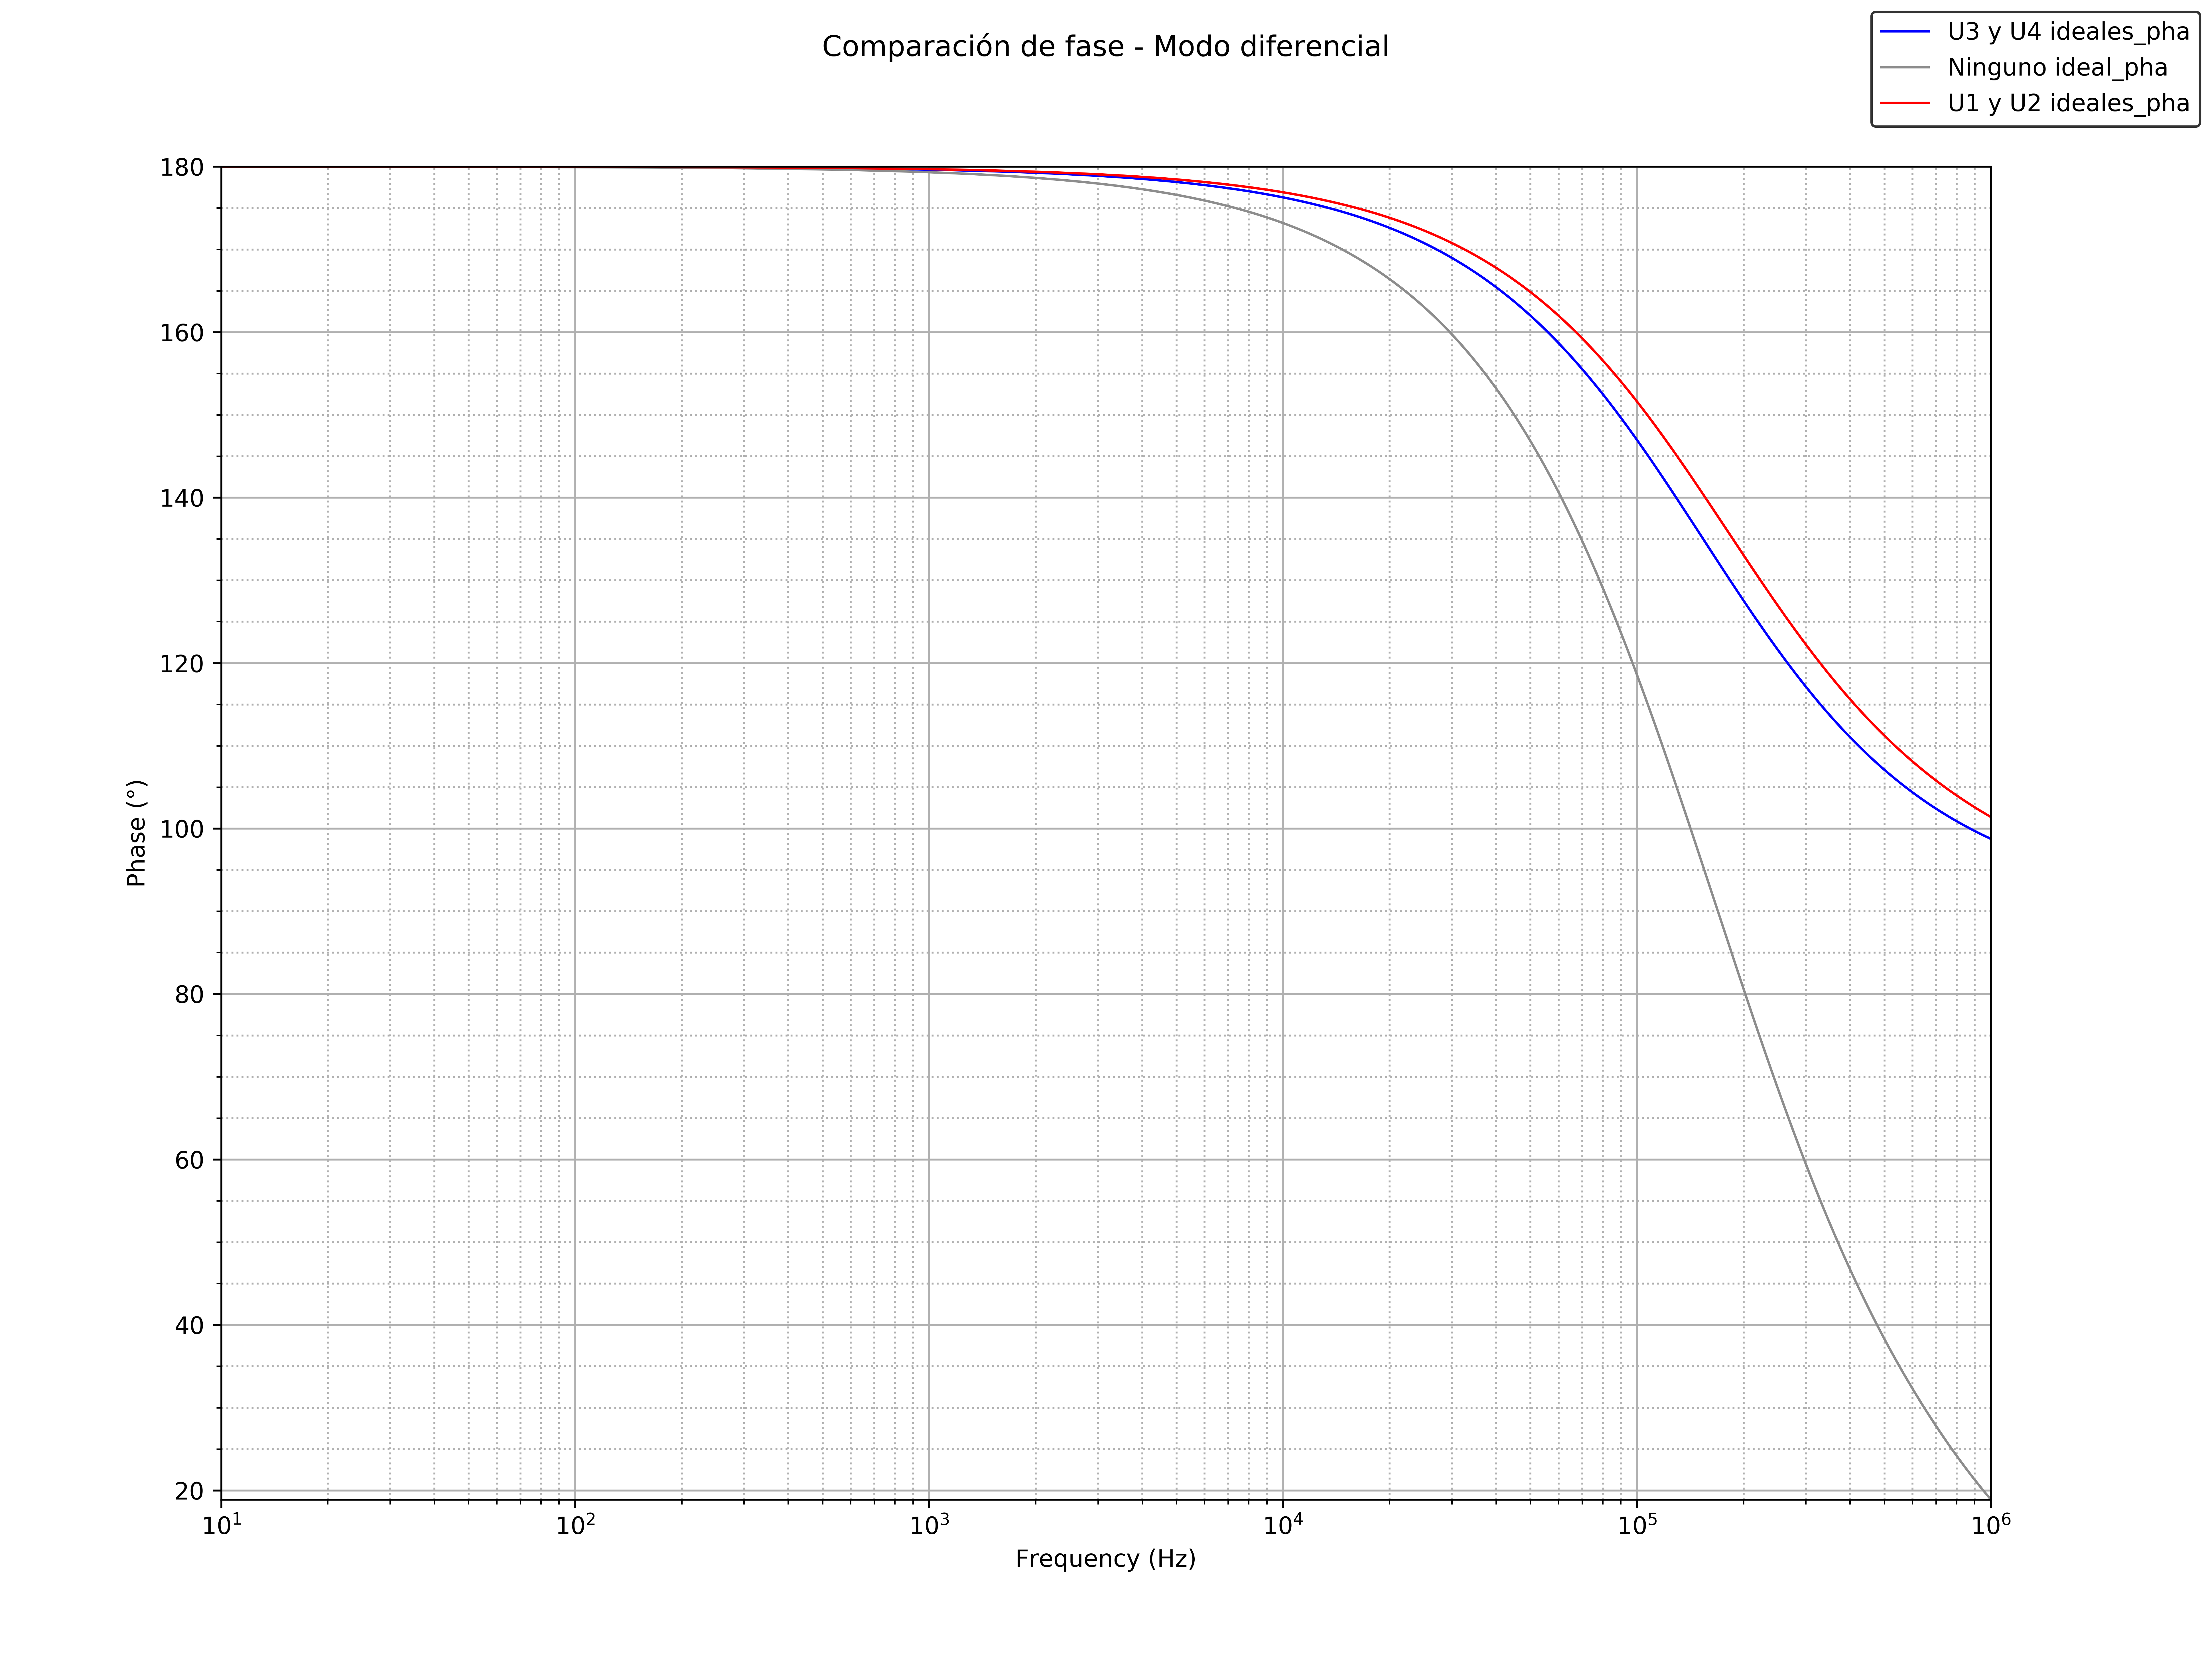
\includegraphics{../EJ3/Recursos/Comp_pha_diff}

\end{tabular}%
}
\caption{Comparaci\'on de M\'odulo y fase de la trasferencia para el amplificador en modo diferencial}
\label{fig:Comp_diff}
\end{figure}

\begin{figure}[H]
    \centering
\resizebox{\textwidth}{!}{%
\begin{tabular}{c c}
    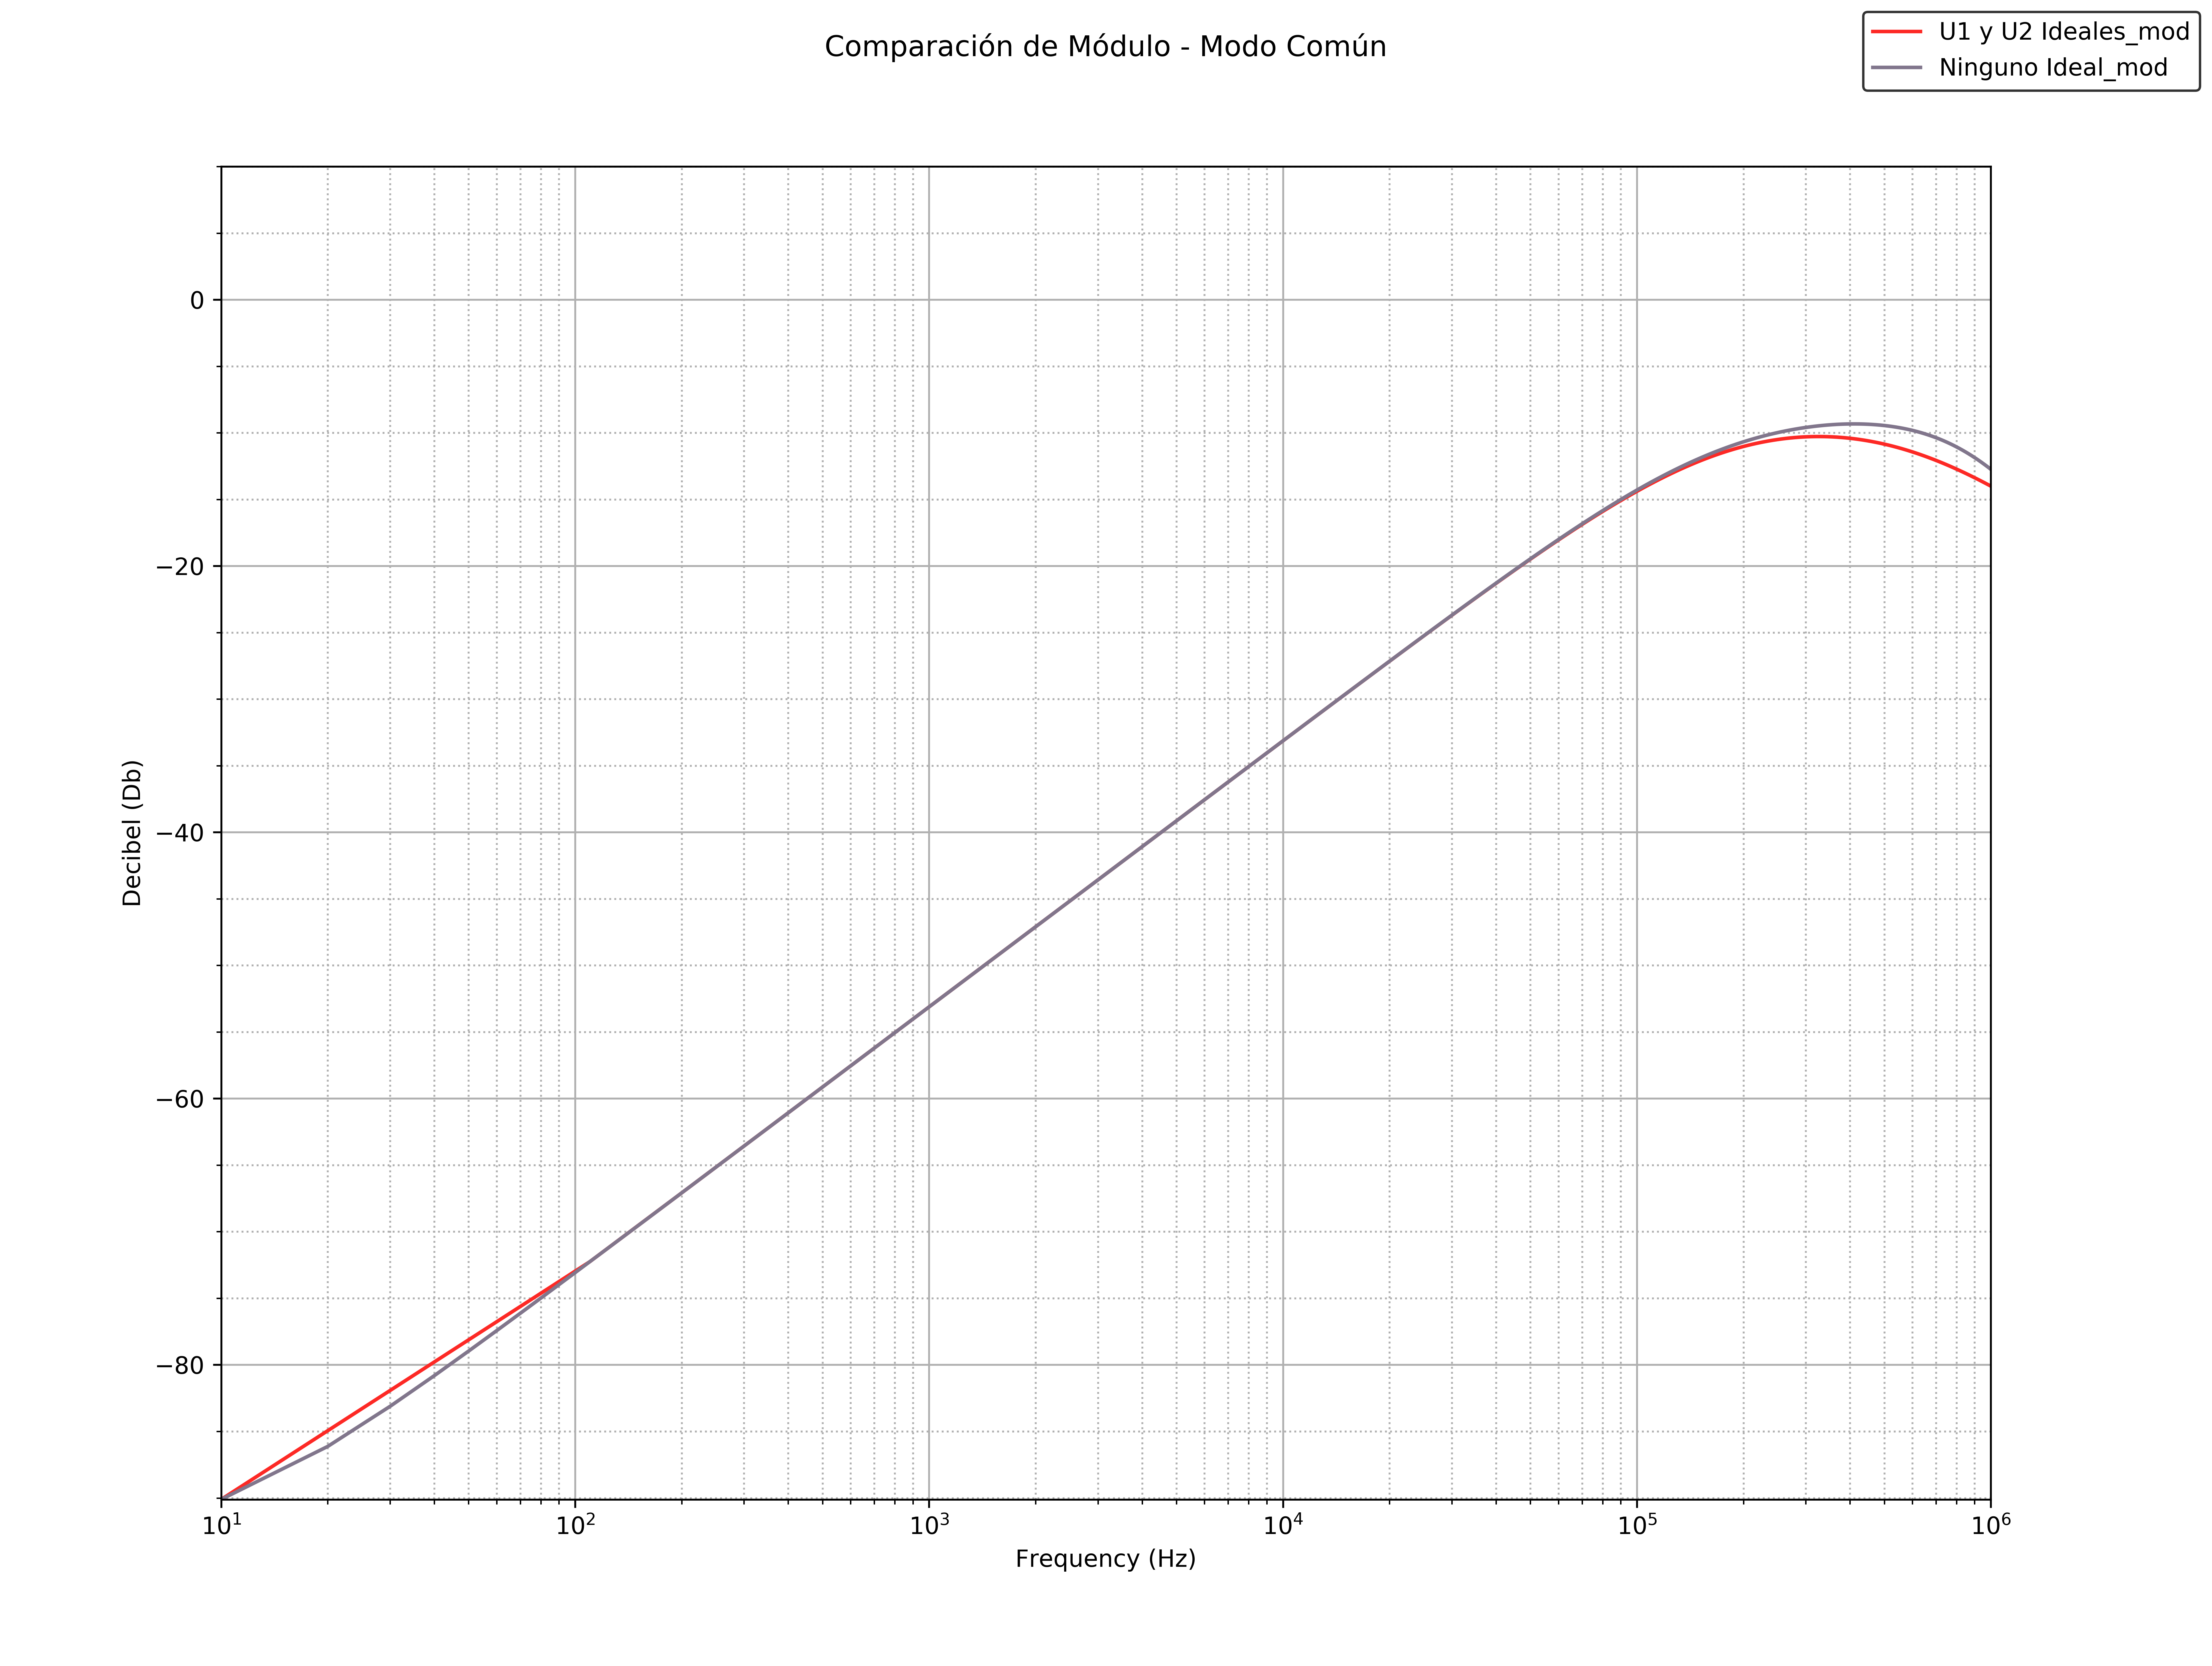
\includegraphics{../EJ3/Recursos/Comp_mod_common} &
    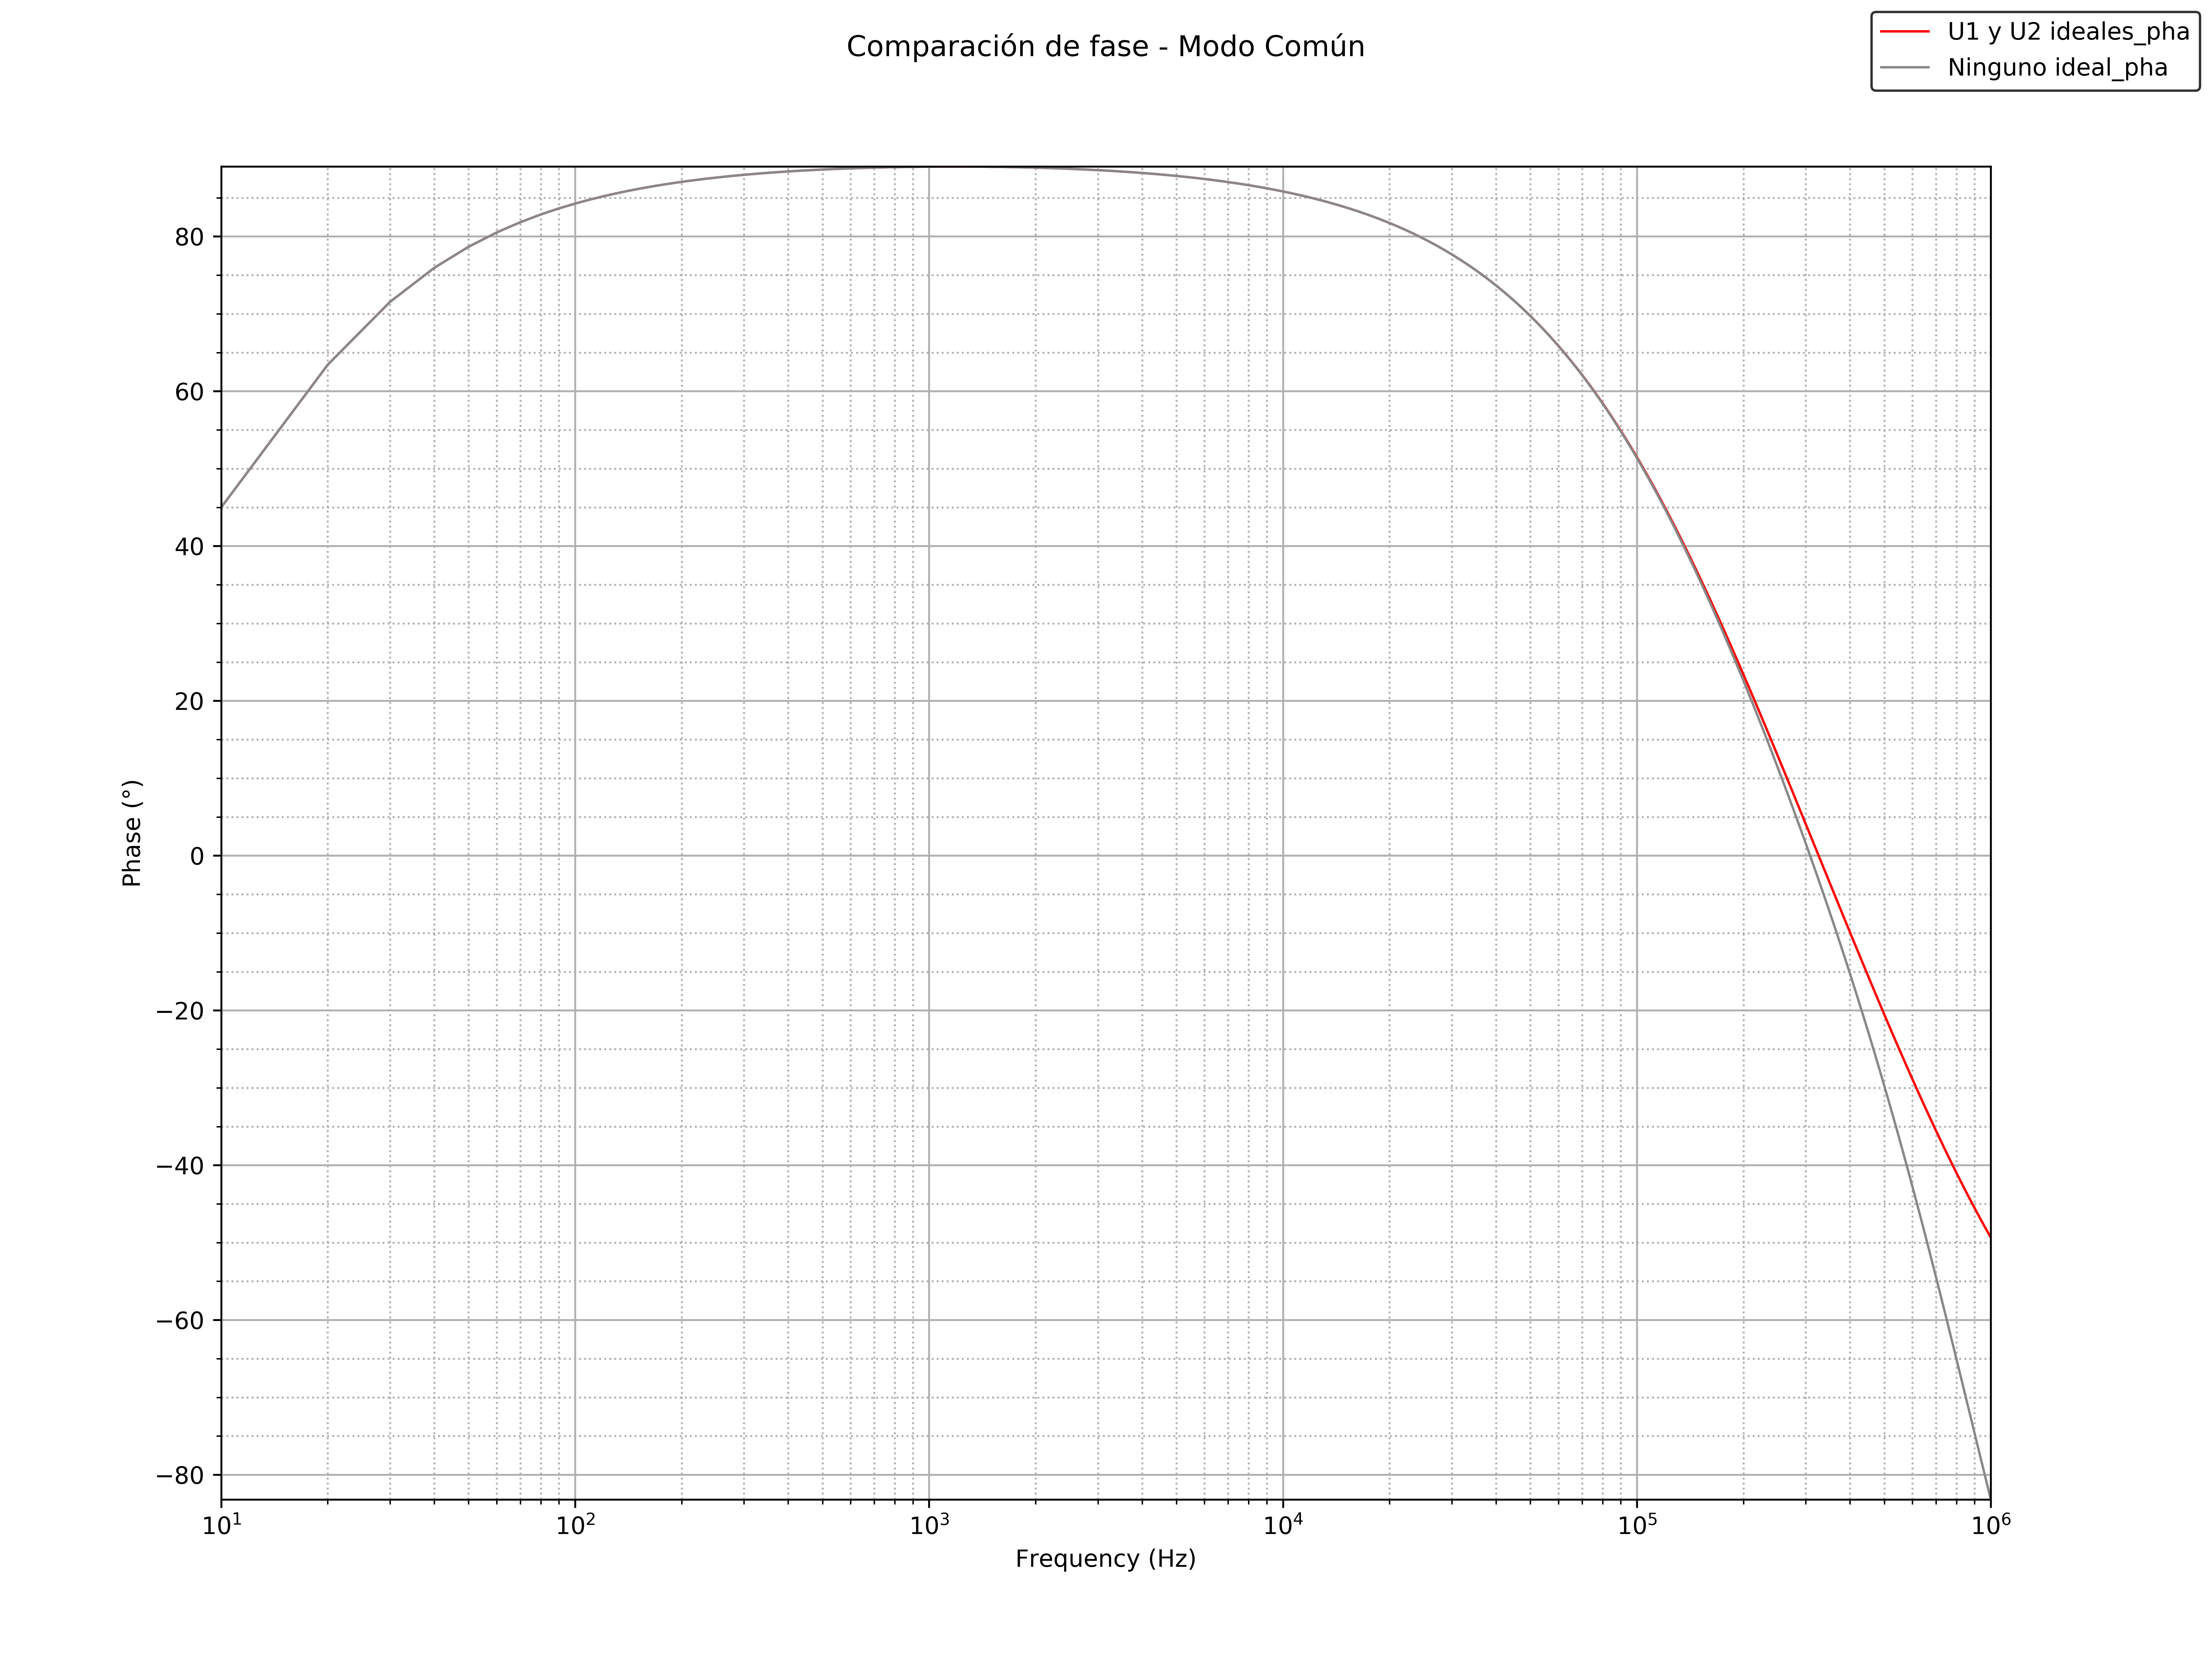
\includegraphics{../EJ3/Recursos/Comp_pha_common}

\end{tabular}%
}
\caption{Comparaci\'on de M\'odulo y fase de la trasferencia para el amplificador en modo com\'un}
\label{fig:Comp_common}
\end{figure}

A partir de los gr\'aficos presentados se puede observar que, como fue mencionado anteriormente, las diferencias entre el TL084 y el amplificador operacional ideal es m\'inima para frecuencias menores a 100KHz.

\subsubsection{An\'alisis de tolerancias, asimentr\'as y variaciones}
Es esta secci\'on se analizan los efectos que provocan las variaciones y asimetr\'ias  de ciertos par\'ametros del amplificador en su comportamiento en funci\'on de la frecuencia. Se verifica que las variaciones para el circuito en modo diferencial son despreciables para la pr\'actica, por lo que solo se presentan los resultados obtenidos en modo com\'un, en donde si pueden notarse las variaciones que son de inter\'es . 

\paragraph{Variaciones de $R_5$:}
$R_5$ es la resistencia que controla la estabilidad del circuito, el rango de valores que esta puede tomar para que el circuito funcione correctamente es acotado. Sin embargo no es posible ver esto desde el an\'alisis te\'orico. Se procede, entonces, a hacer un barrido por distintos valores para esta resistencia para verificar que valor elegido para ser utilizado sea el correcto. 
El resultado de este proceso se muestra en la Figura \ref{fig:Comp_common_R5}.
\begin{figure}[H]
    \centering
\resizebox{\textwidth}{!}{%
\begin{tabular}{c c}
    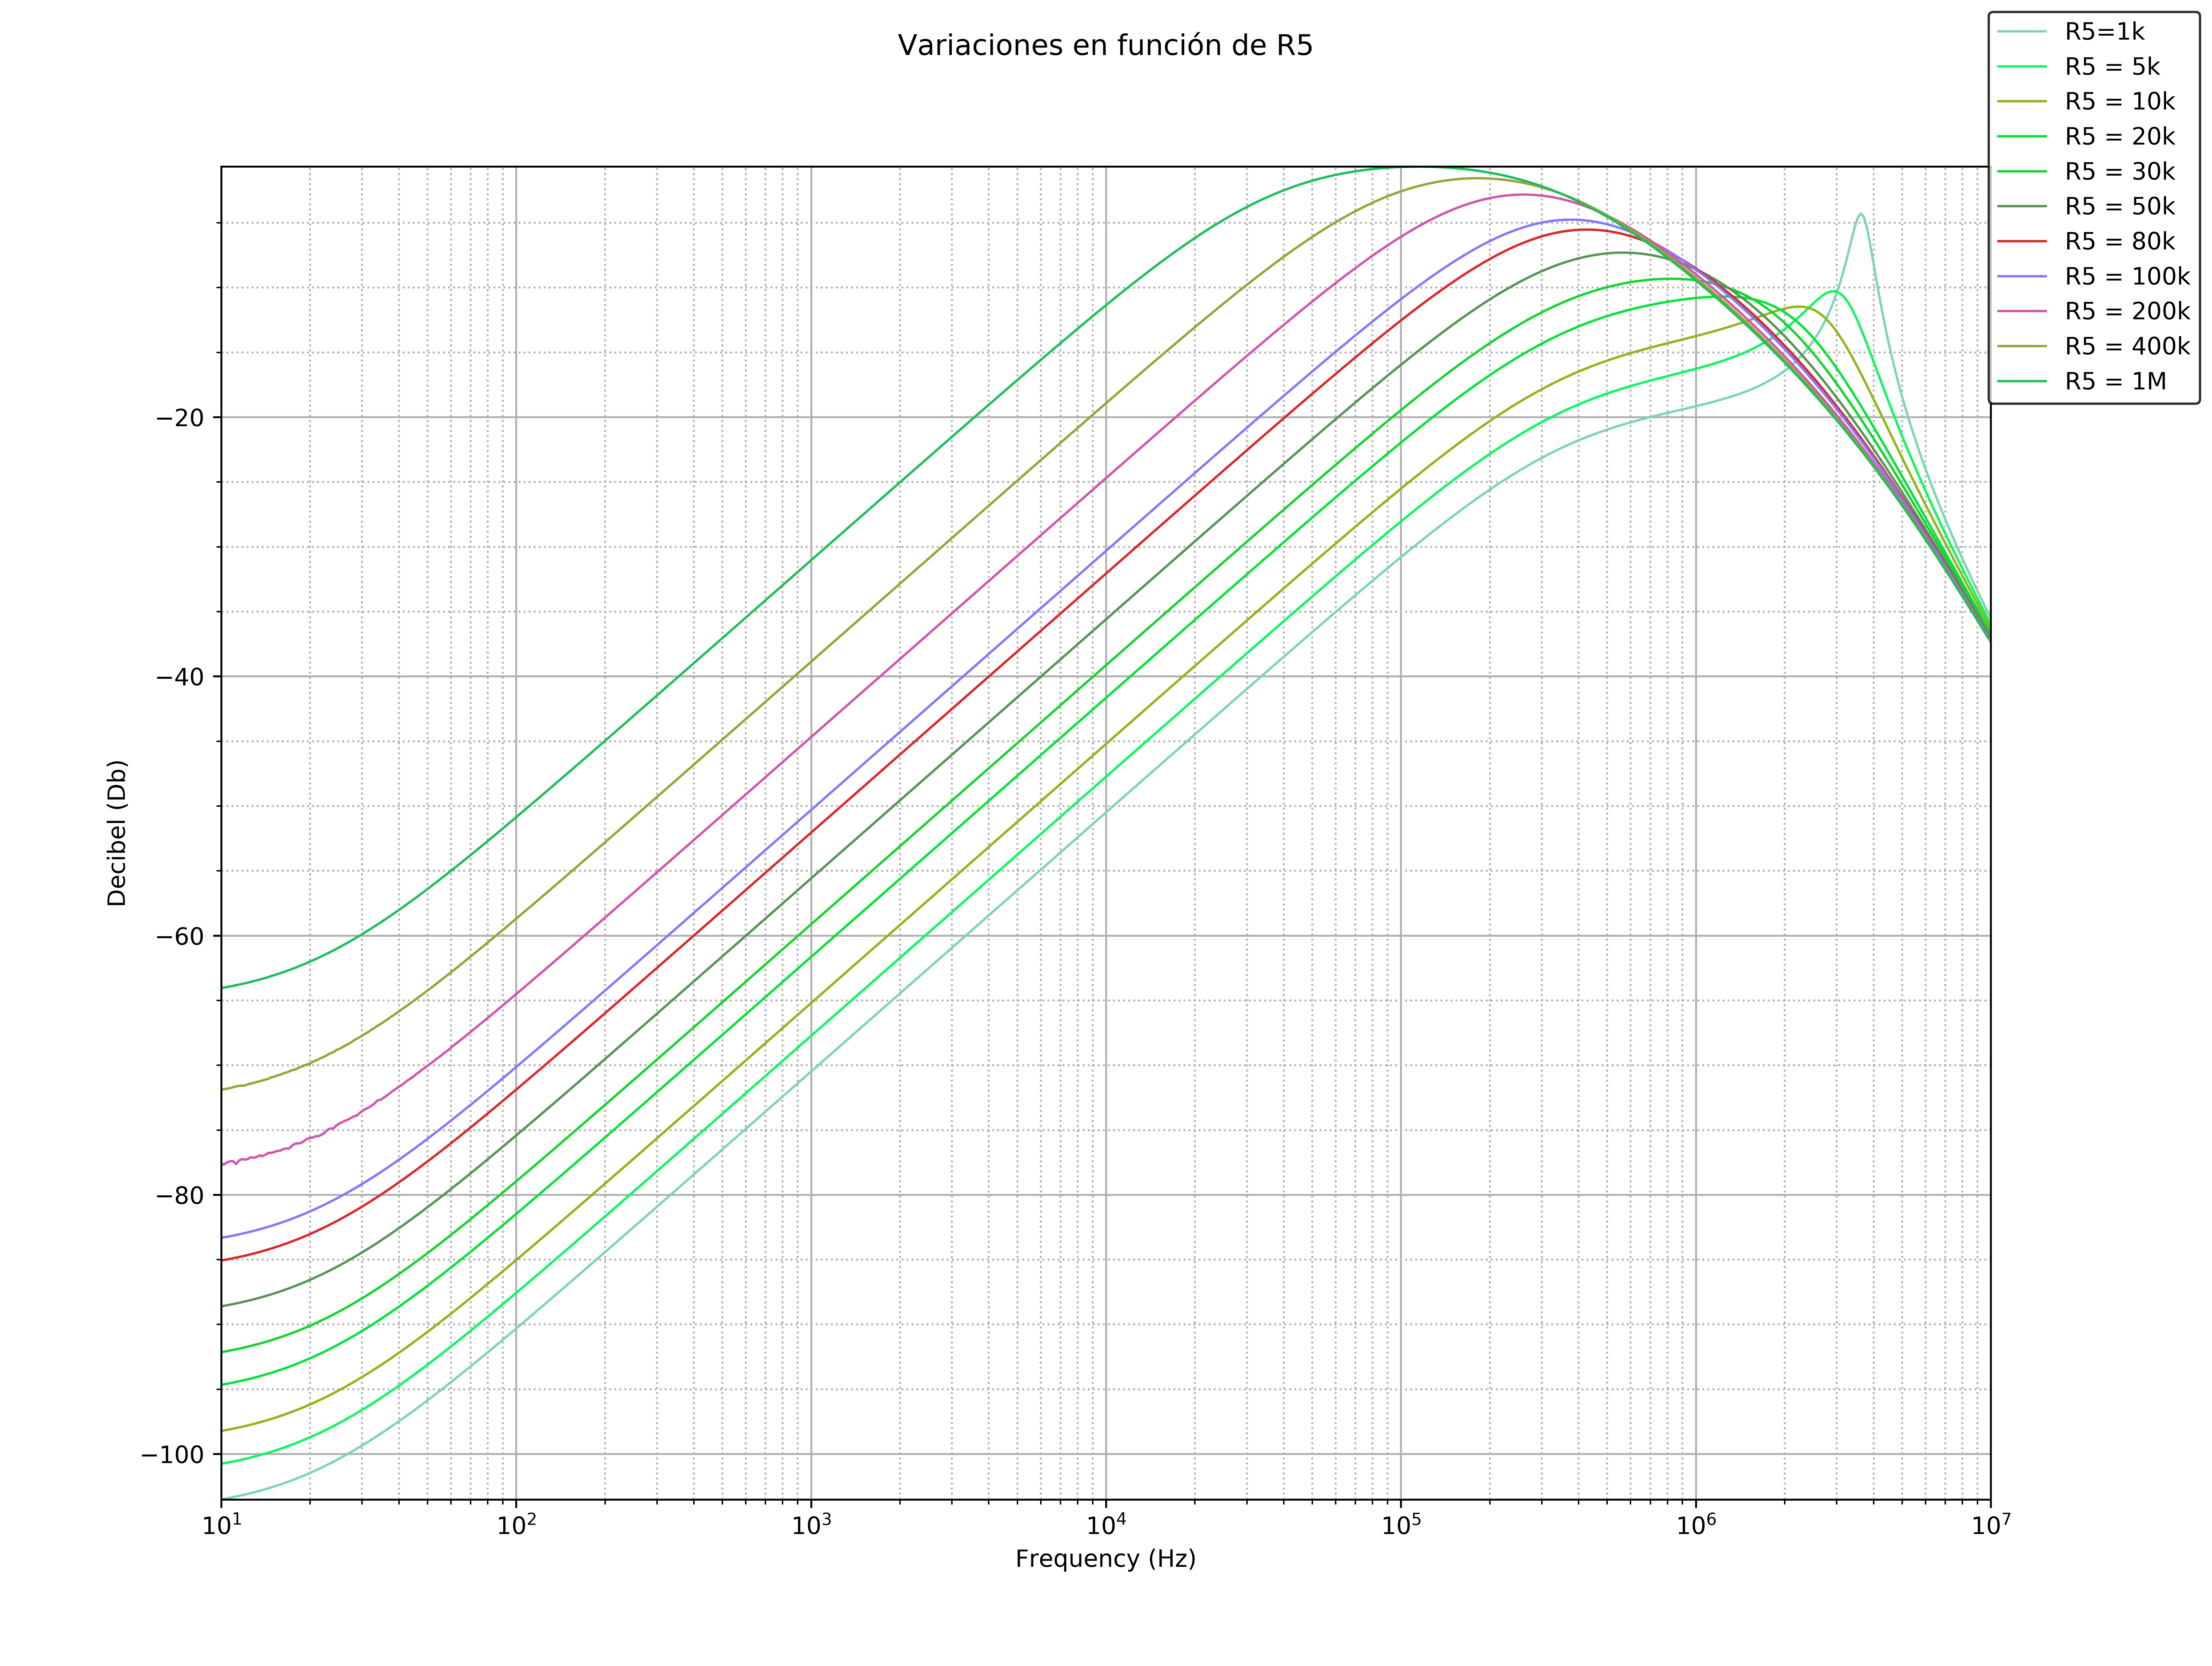
\includegraphics{../EJ3/Recursos/varR5_mod_common} &
    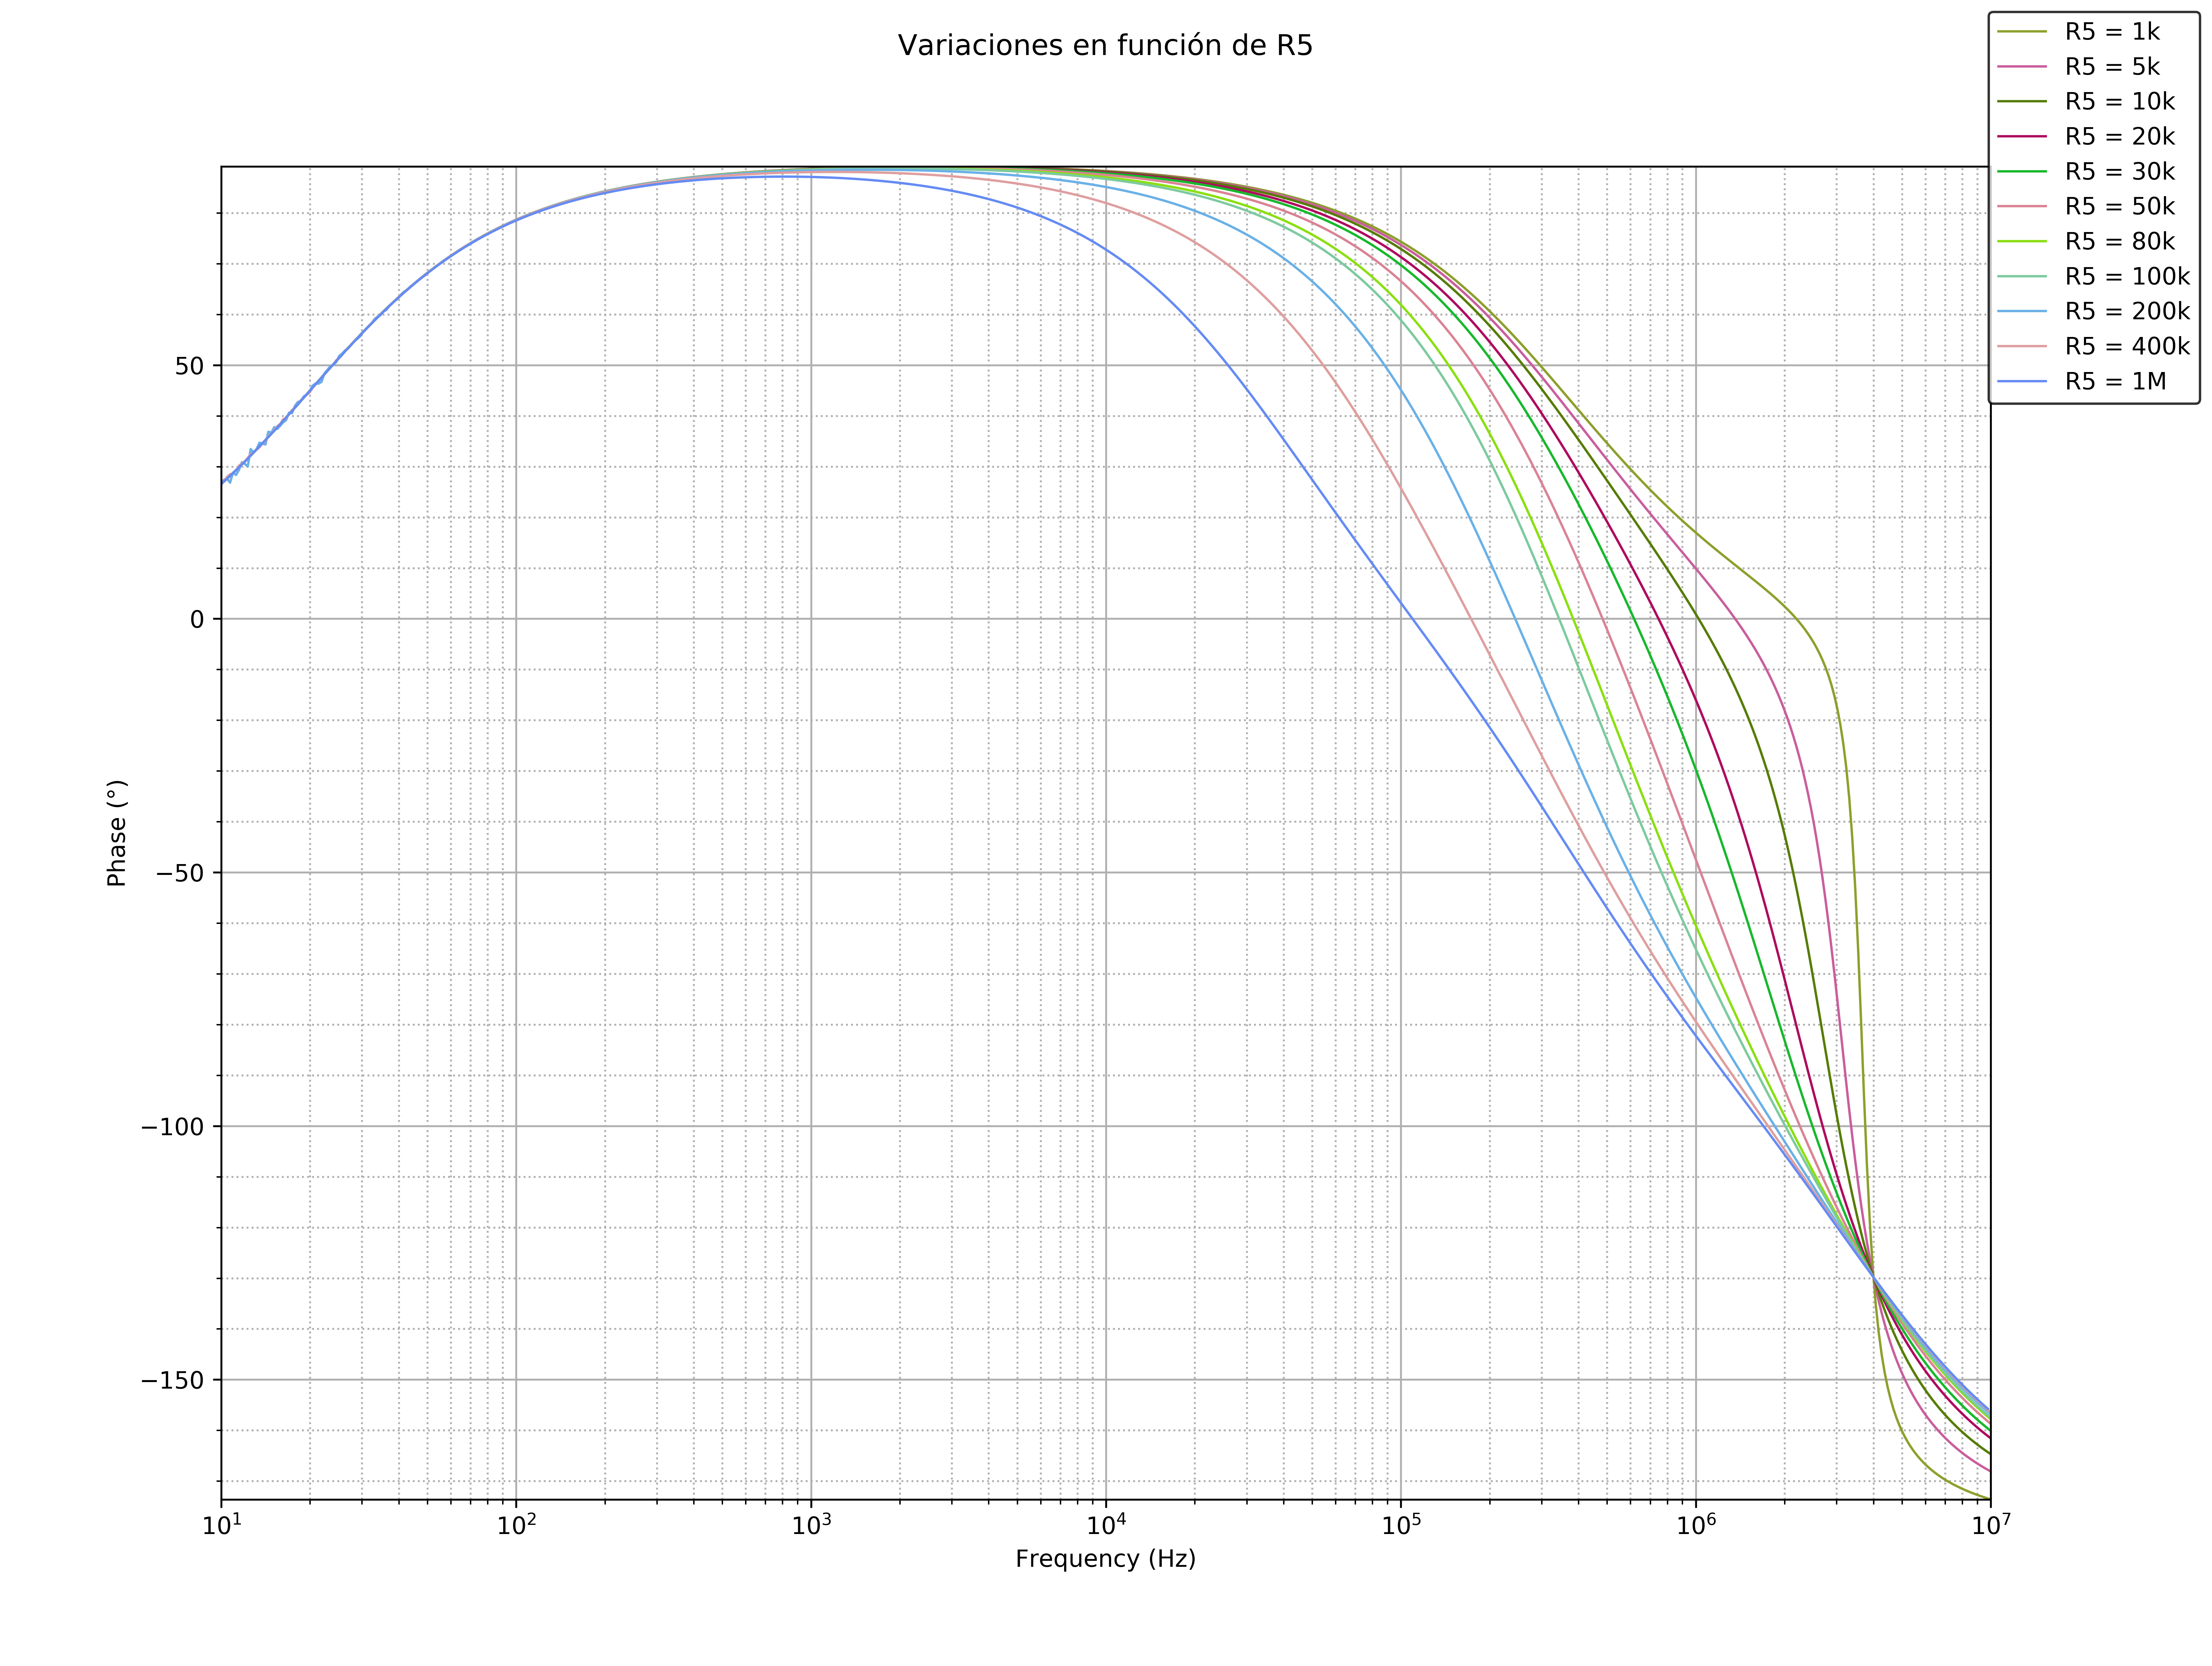
\includegraphics{../EJ3/Recursos/varR5_pha_common}

\end{tabular}%
}
\caption{Comparaci\'on de M\'odulo y fase de la trasferencia para el amplificador en modo com\'un}
\label{fig:Comp_common_R5}
\end{figure}

\paragraph{Tolerancias y asimetr\'ias de $R_3$, $R_4$, $R_6$ y $R_7$:}
Se realiza para este caso un an\'alisis Monte Carlo, para estas resistencias con tolerancia del 1\%. Nuevamente se verifica que las variaciones para el circuito en modo diferencial son desprecibles, por lo que solo se presentan los resultados obtenidos en modo com\'un, en donde si pueden notarse las variaciones que son de inte\'es.
Se puede observar en en la Figura \ref{fig:MC_entrada} lo efectos de las variaciones de estas resistencias.
\begin{figure}[H]
    \centering
\resizebox{\textwidth}{!}{%
\begin{tabular}{c c}
    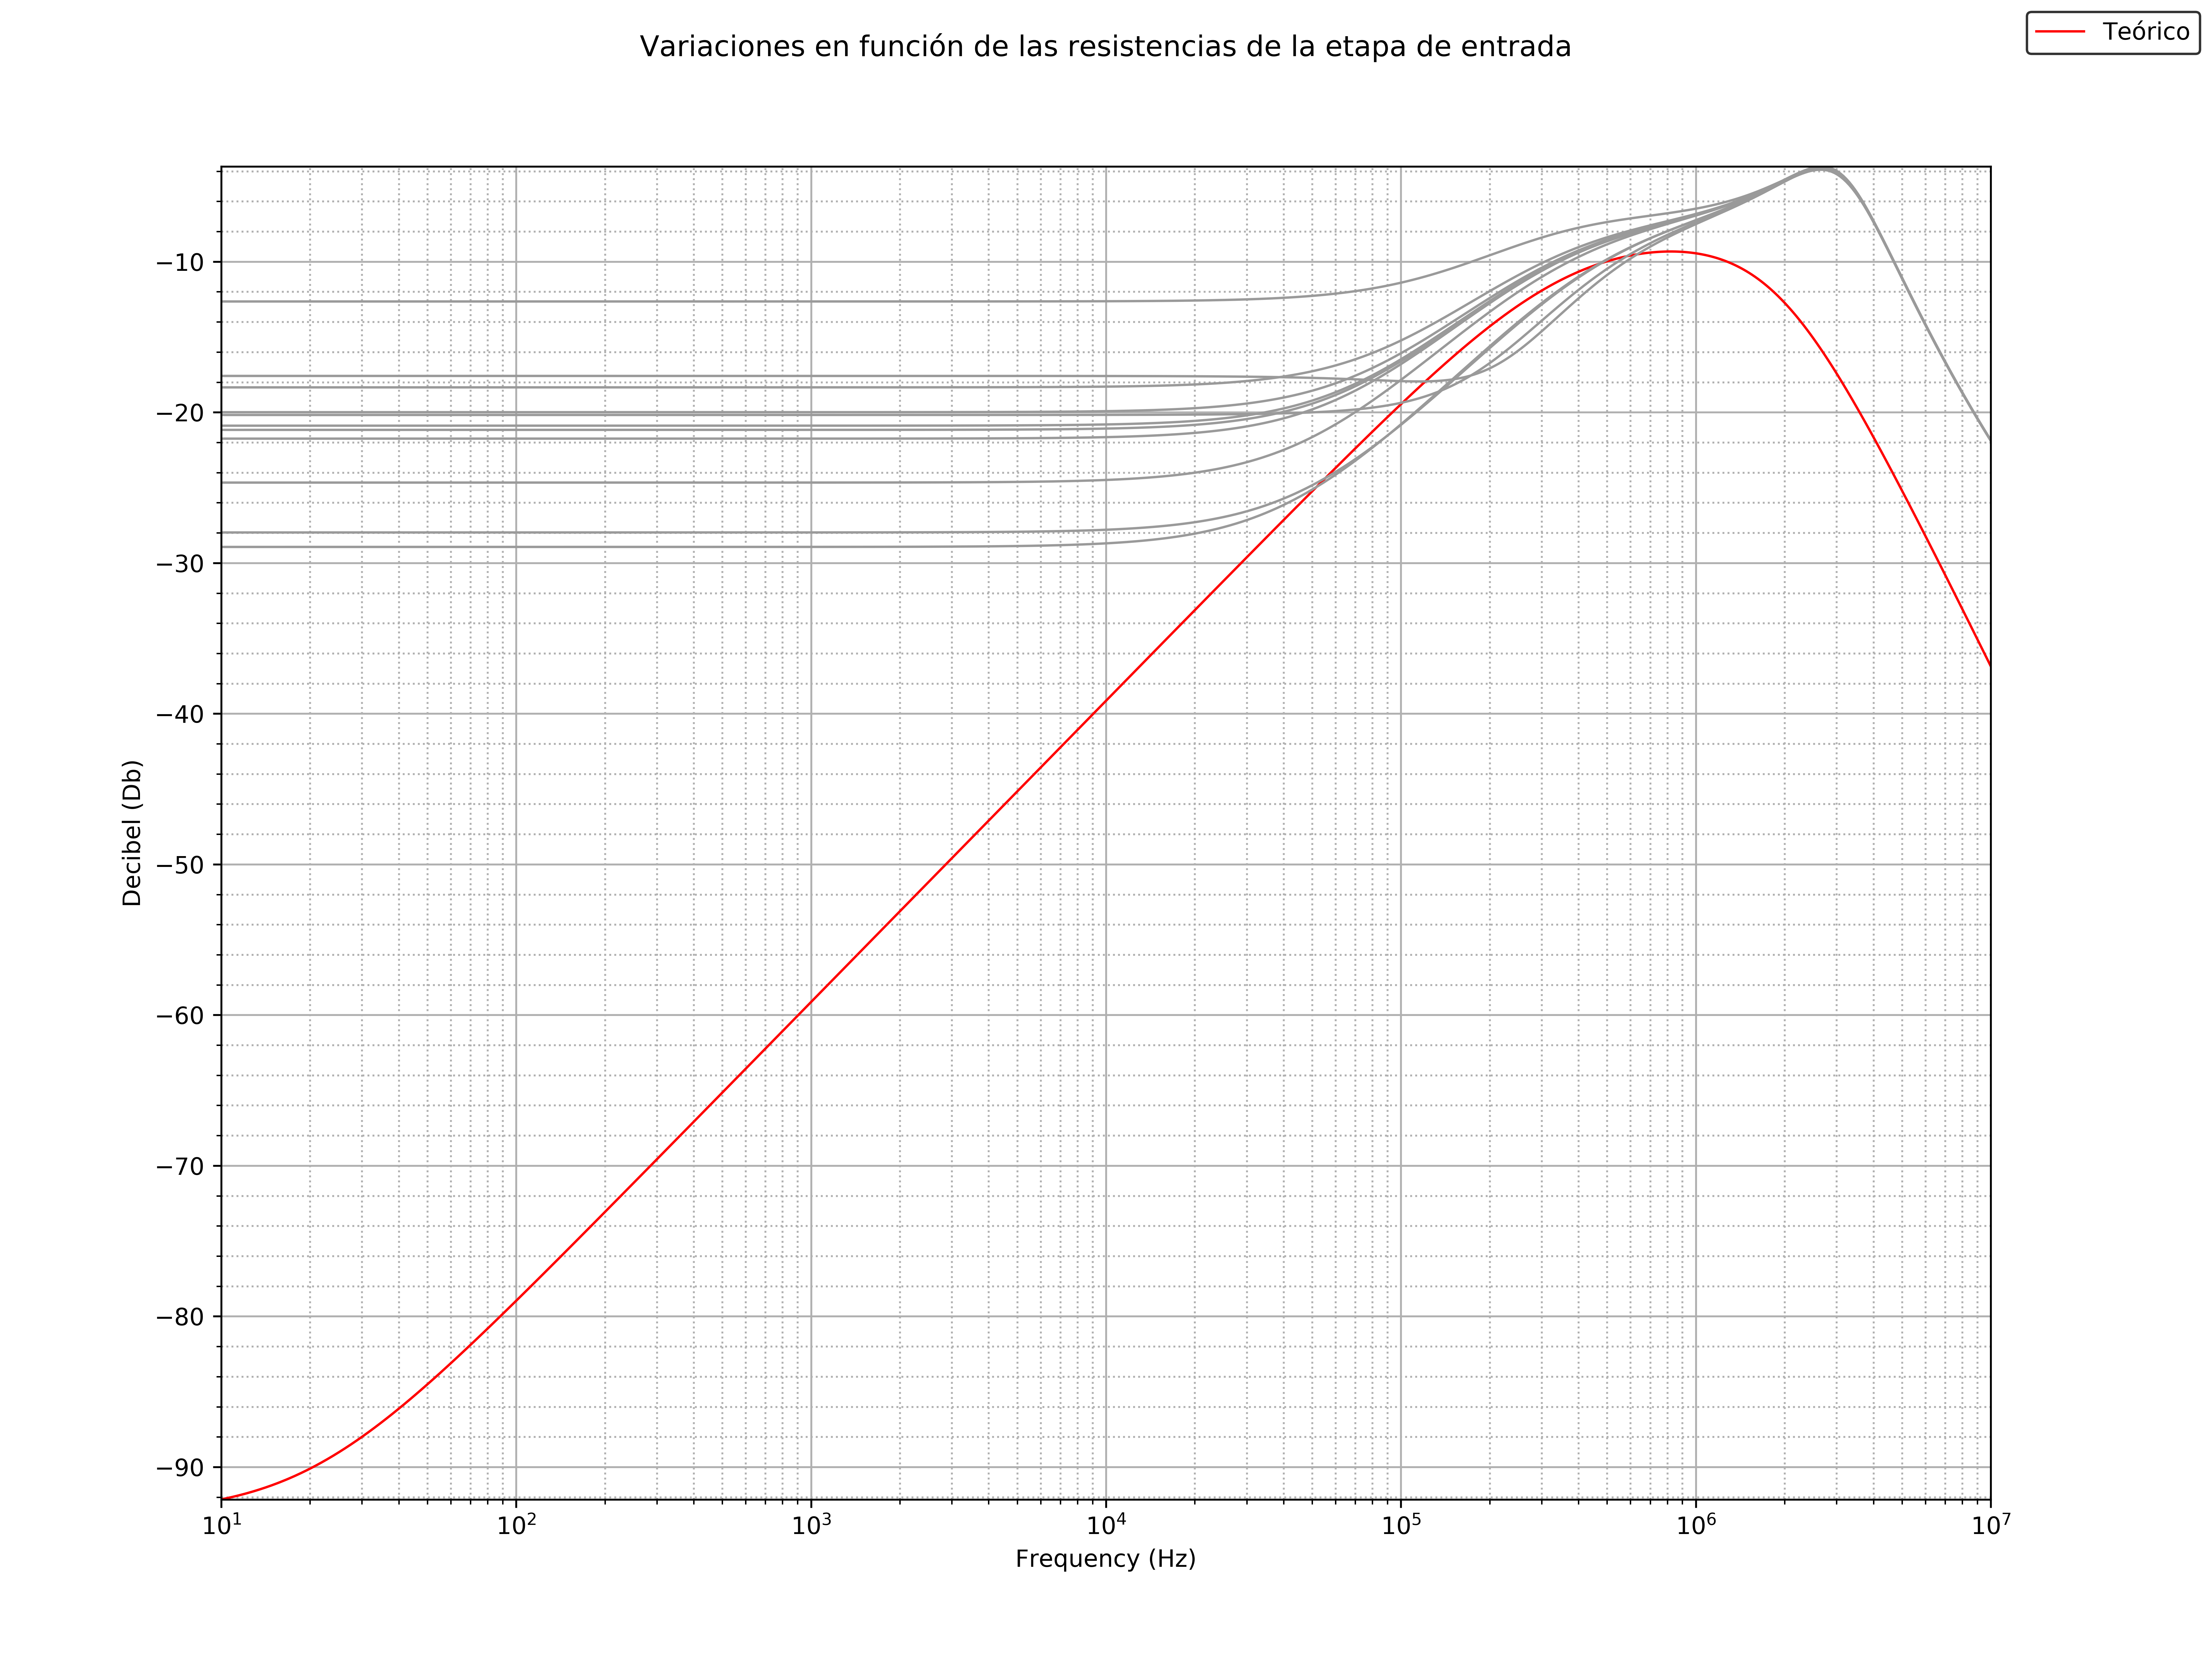
\includegraphics{../EJ3/Recursos/MC_ent} &
    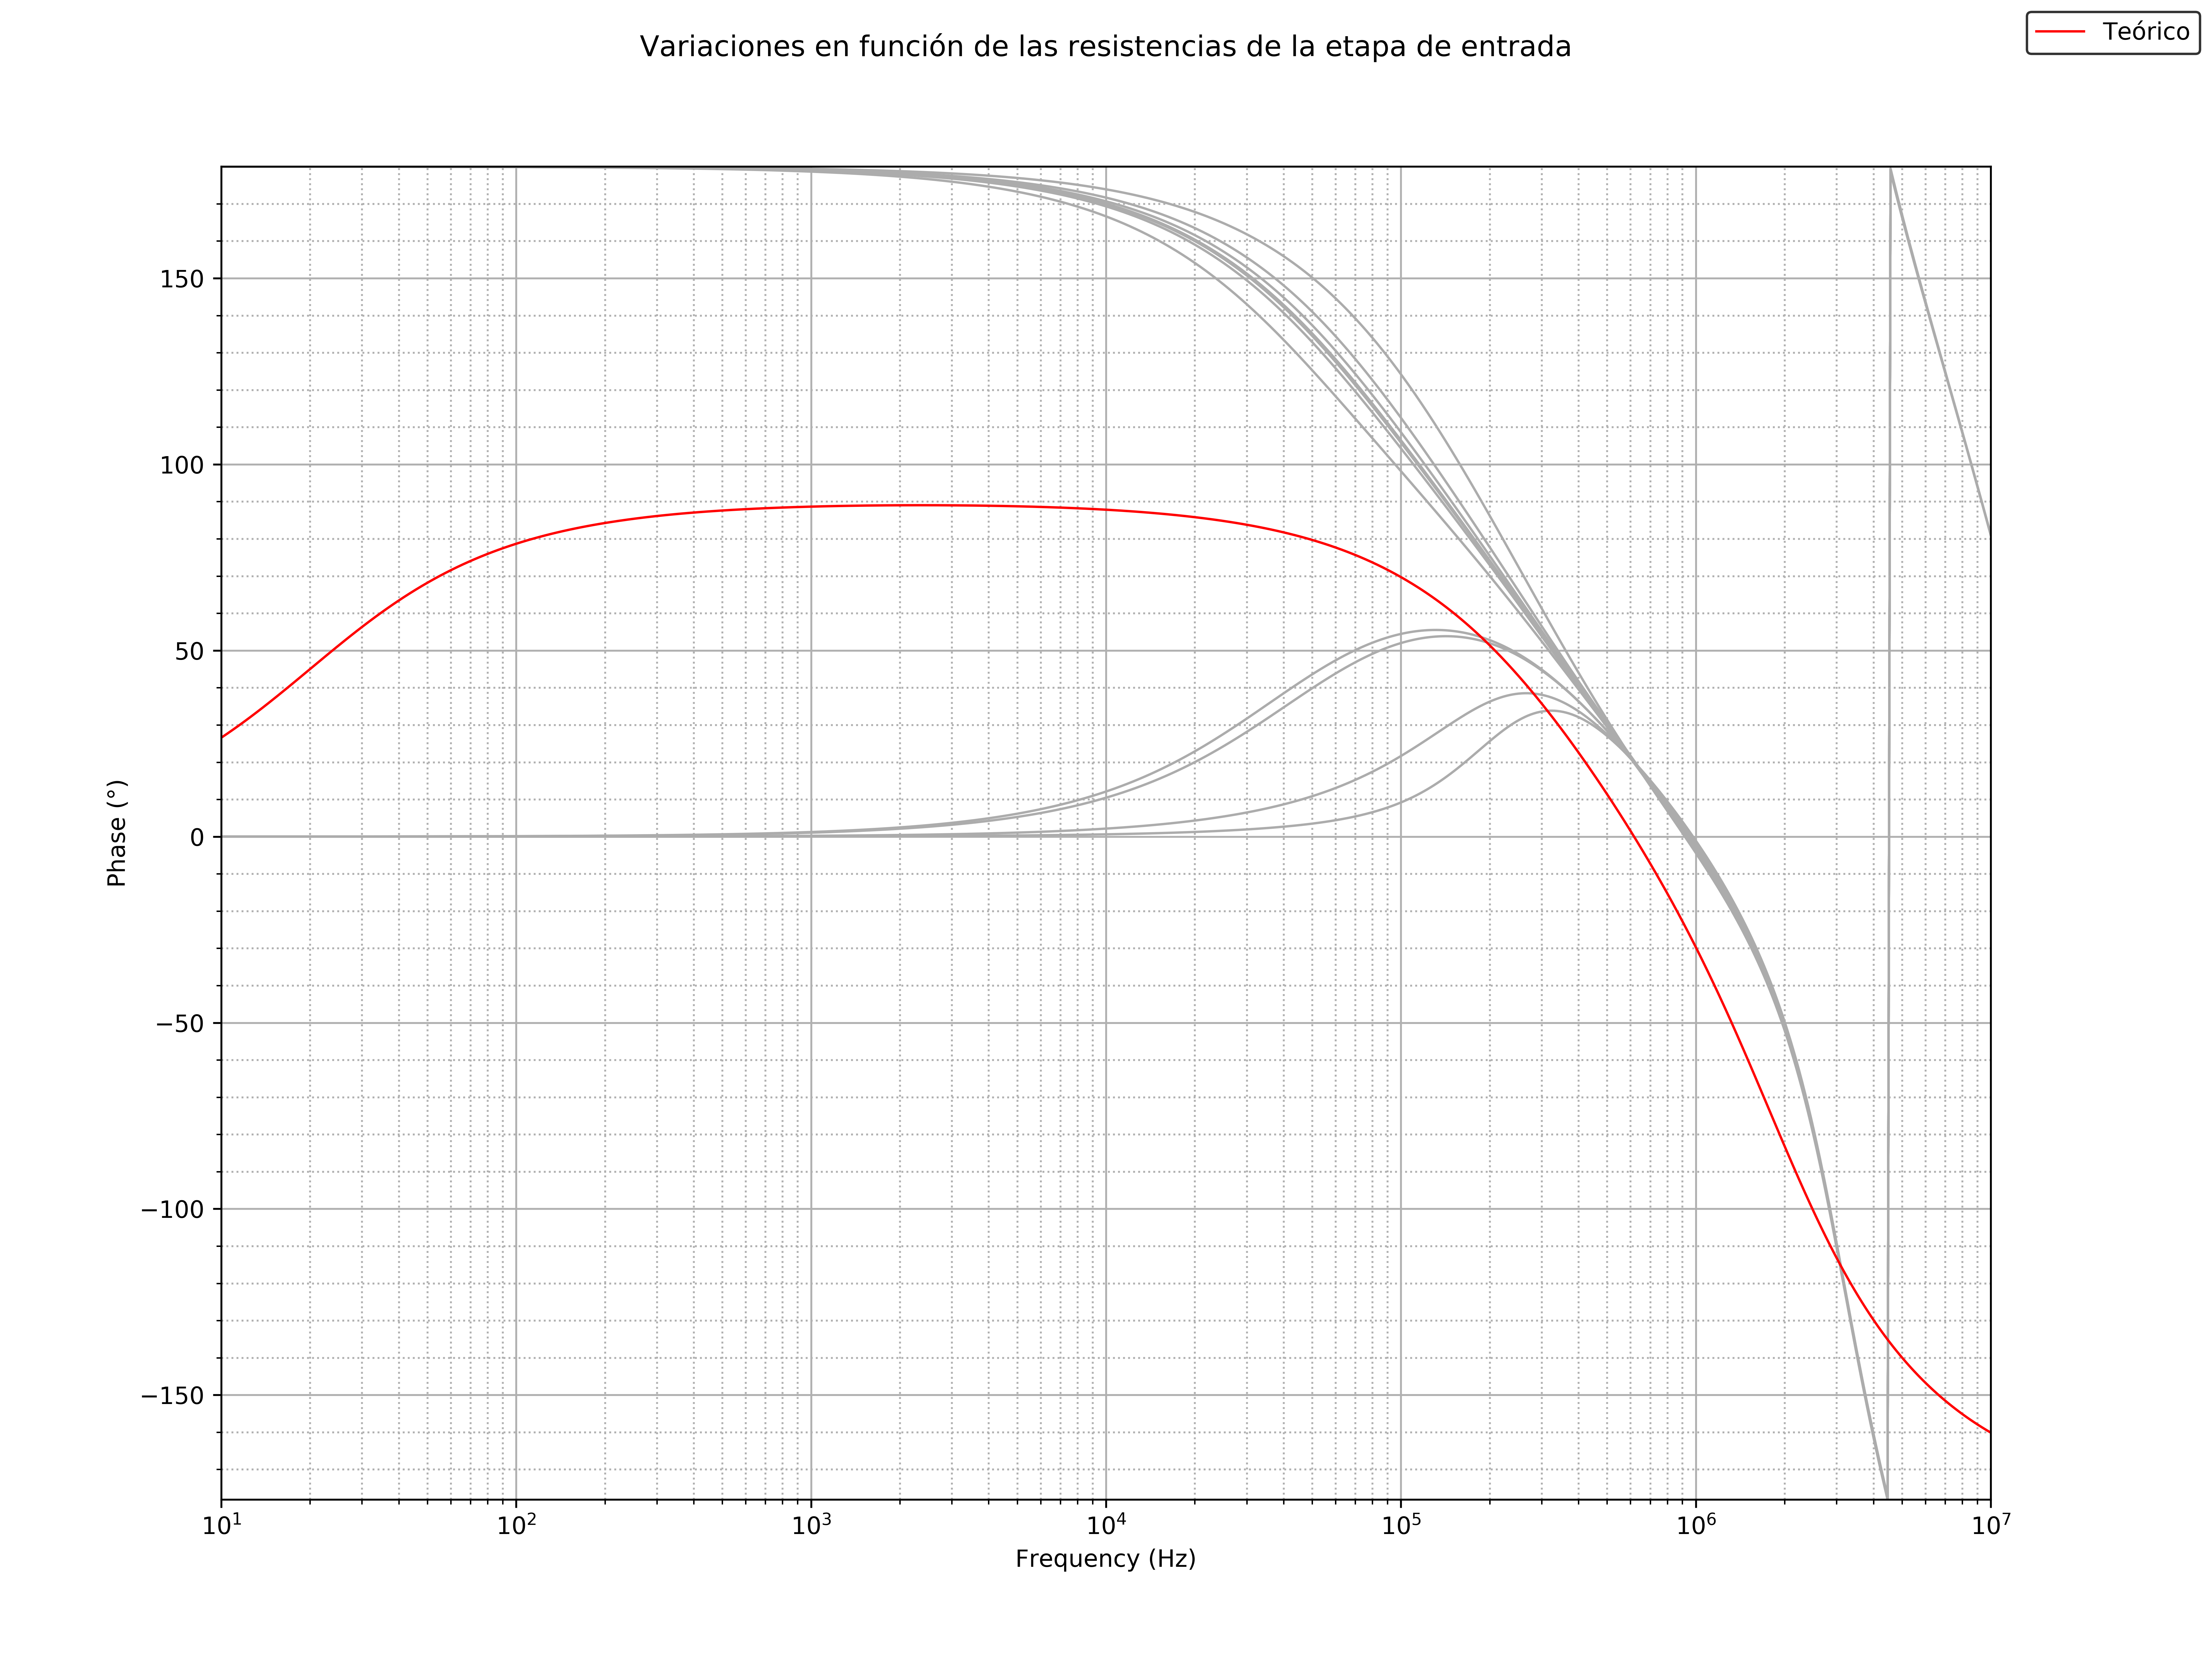
\includegraphics{../EJ3/Recursos/MC_ent_pha}

\end{tabular}%
}
\caption{Comparaci\'on de M\'odulo y fase de la trasferencia para el amplificador en modo com\'un}
\label{fig:MC_entrada}
\end{figure}
En este caso se muestran en gris en an\'alisis de las variaciones en el modelo de LTSpice del fabricante en relaci\'on al te\'orico calculado en la secci\'on anterior. En este caso se observa una mayor variaci\'on. En base a estas diferencias se concluye que el modelo utilizado pra realizar las simulaciones tiene en cuenta m\'as efectos que los considerados para el an\'alisis te\'orico realizado.
\paragraph{Variaciones de $A_o$ y GBP}
Para analizar como afectan las variaciones de estos par\'ametrs, se sigue el siguiente procedimiento. Utilizando como limites los valores m\'inimos y t\'ipicos(debido a que no se provee el m\'aximo) de la hoja de datos del fabricante se procede a hacer un barrido lineal analizando las desviaciones para los distintos valores posibles.
Para este an\'alisis se utiliza el modelo de amplificador operacional configurable de LTSpice y no el an\'alsis te\'orico.
Se puede observar en en la Figura \ref{fig:VAR_AoyGBP} lo efectos de las variaciones de estas resistencias.
\begin{figure}[H]

    \centering
    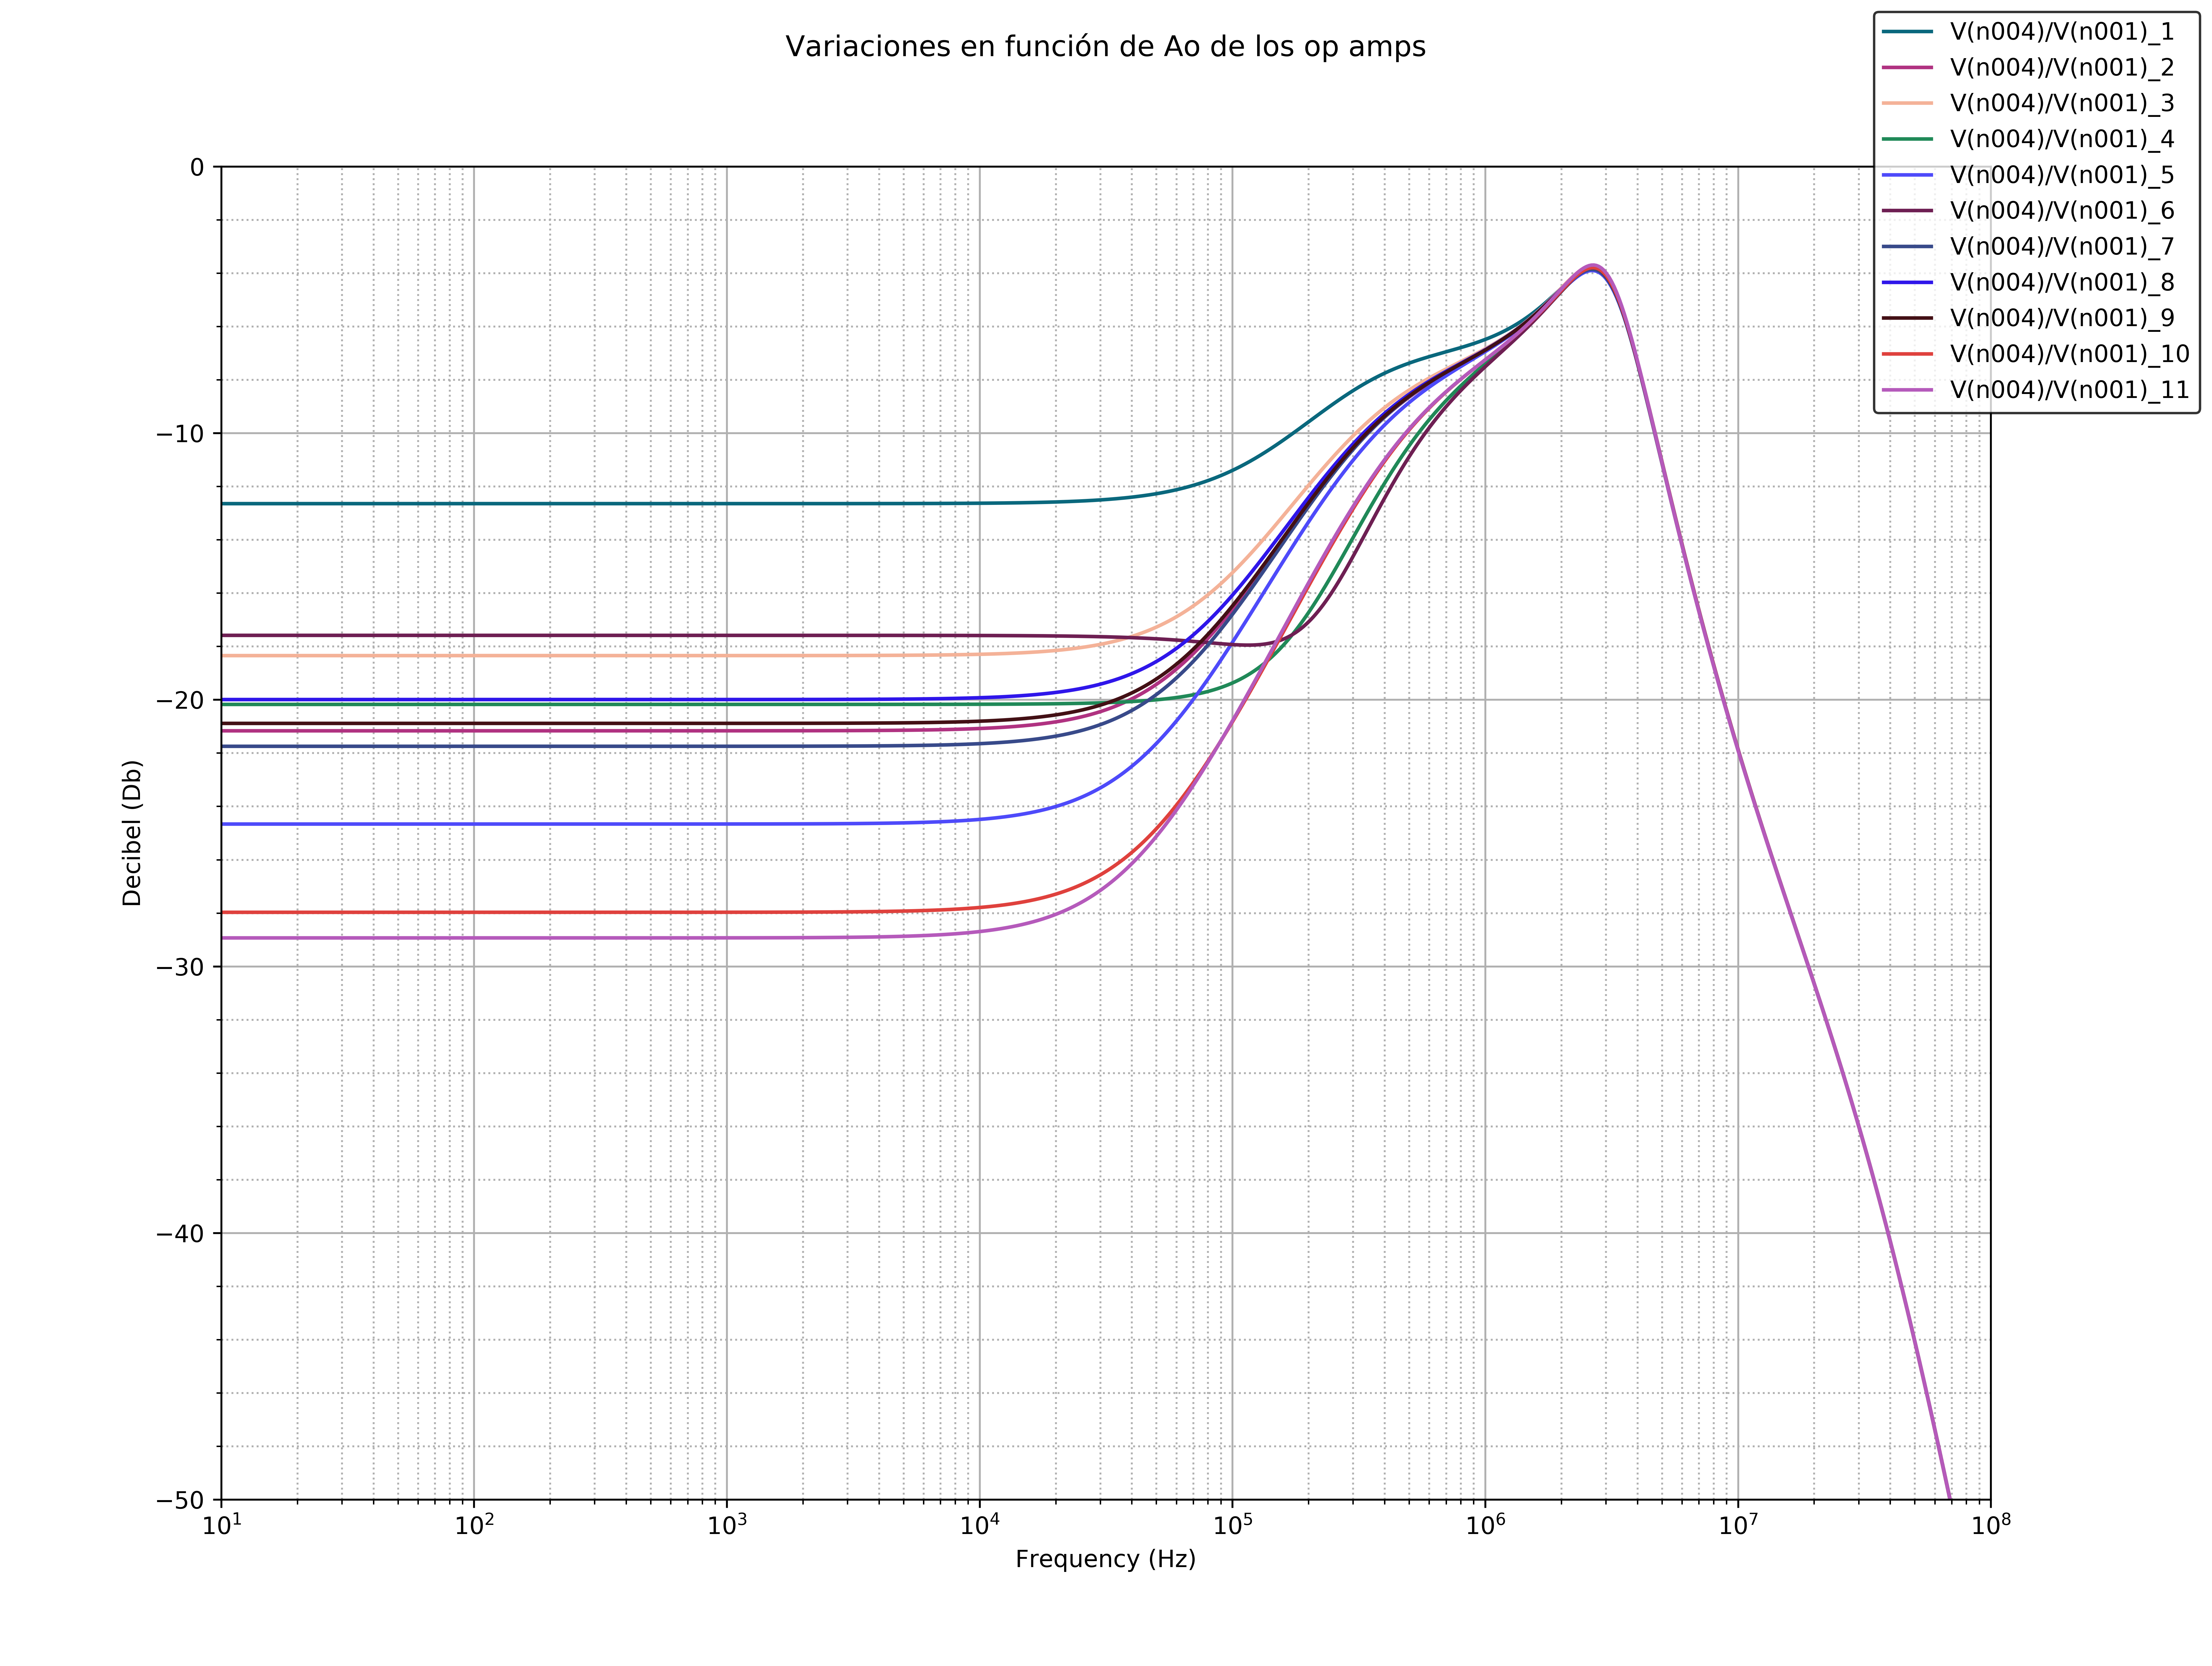
\includegraphics[width=0.5\textwidth]{../EJ3/Recursos/VAR_Ao}
    \caption{Transferencia en funci\'on de variaciones de $A_o$ y GBP}
    \label{fig:VAR_AoyGBP}
\end{figure}


\subsubsection{Mediciones y comparaci\'on de resultados}

Se muestra en las Figuras \ref{fig:RES_DIF} y \ref{fig:RES_COM}los gr\'aficos de m\'udulo y fase tanto en modo com\'un como en modo diferencial, con las curvas obtenidas a partir del an\'alisis te\'orico, las simulaciones y las mediciones, a fin de comparar los resultados.
Para el caso del an\'alisis te\'orico se utiliza el caso mas general, que es el c\'alculo realizado con todos los amplificadores operacionales reales. Se utiliza el mismo criterio para las simulaciones.

\begin{figure}[H]
    \centering
\resizebox{\textwidth}{!}{%
\begin{tabular}{c c}
    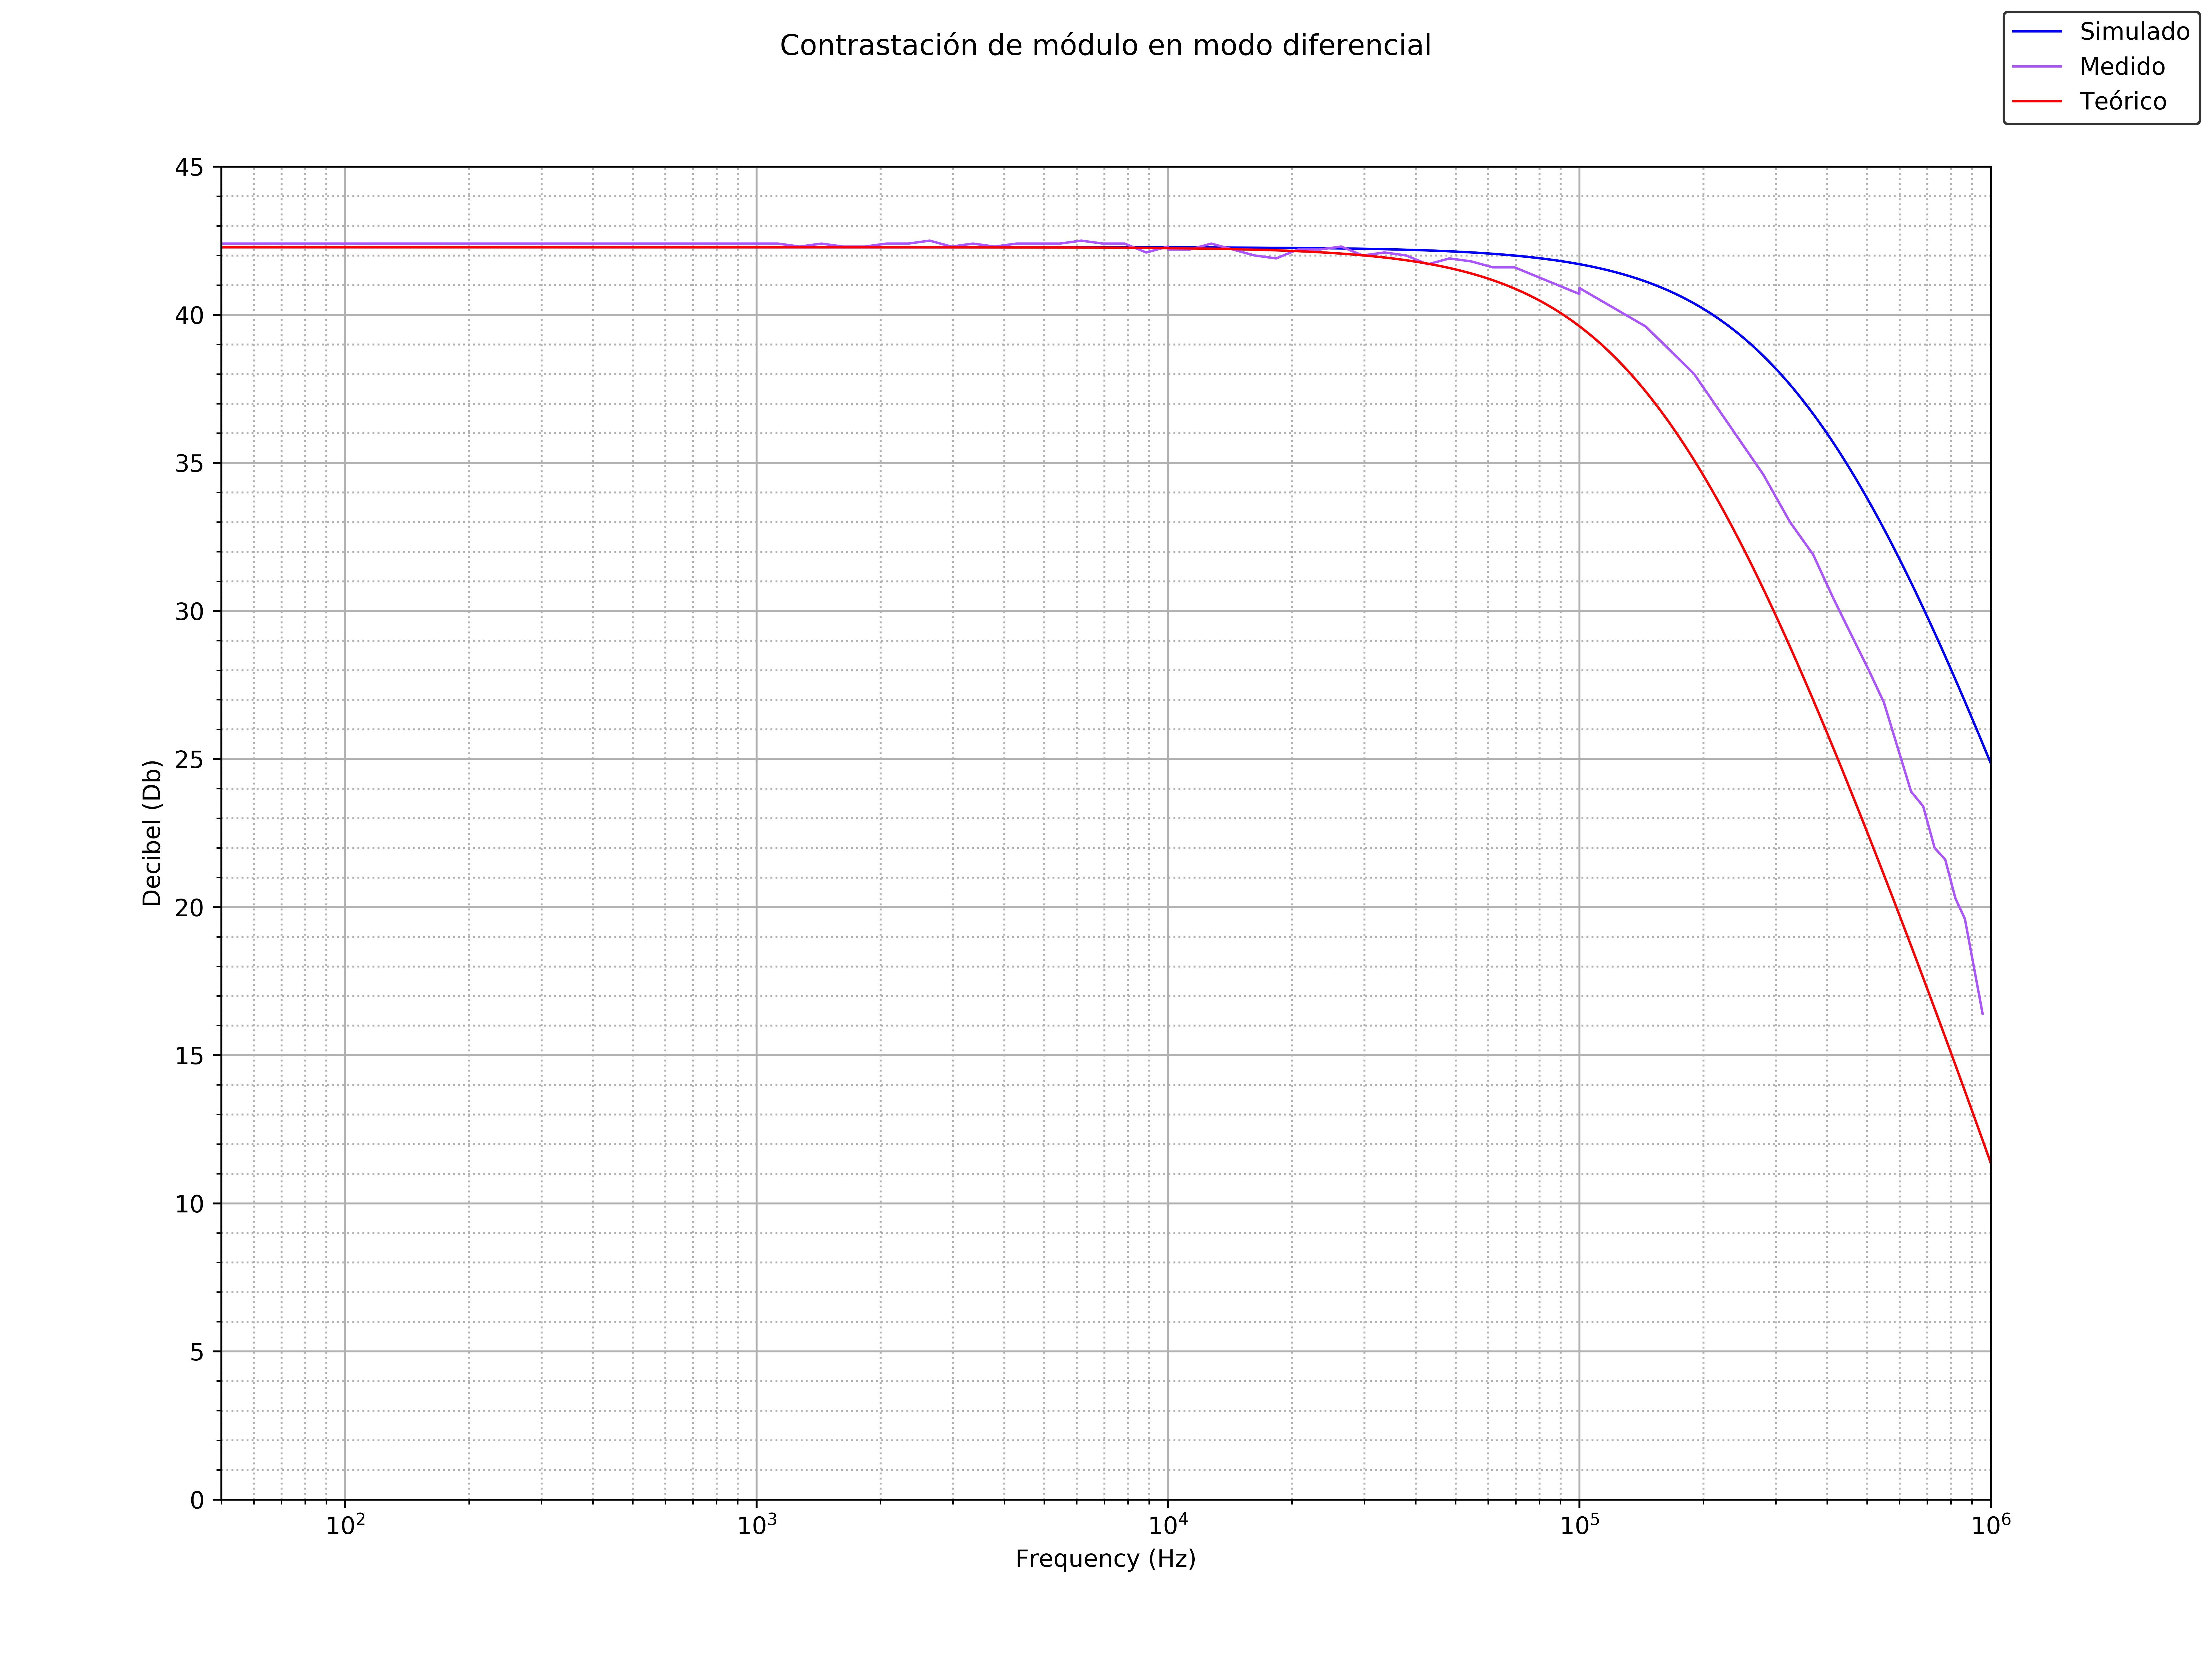
\includegraphics{../EJ3/Recursos/RES_MOD_DIF} &
    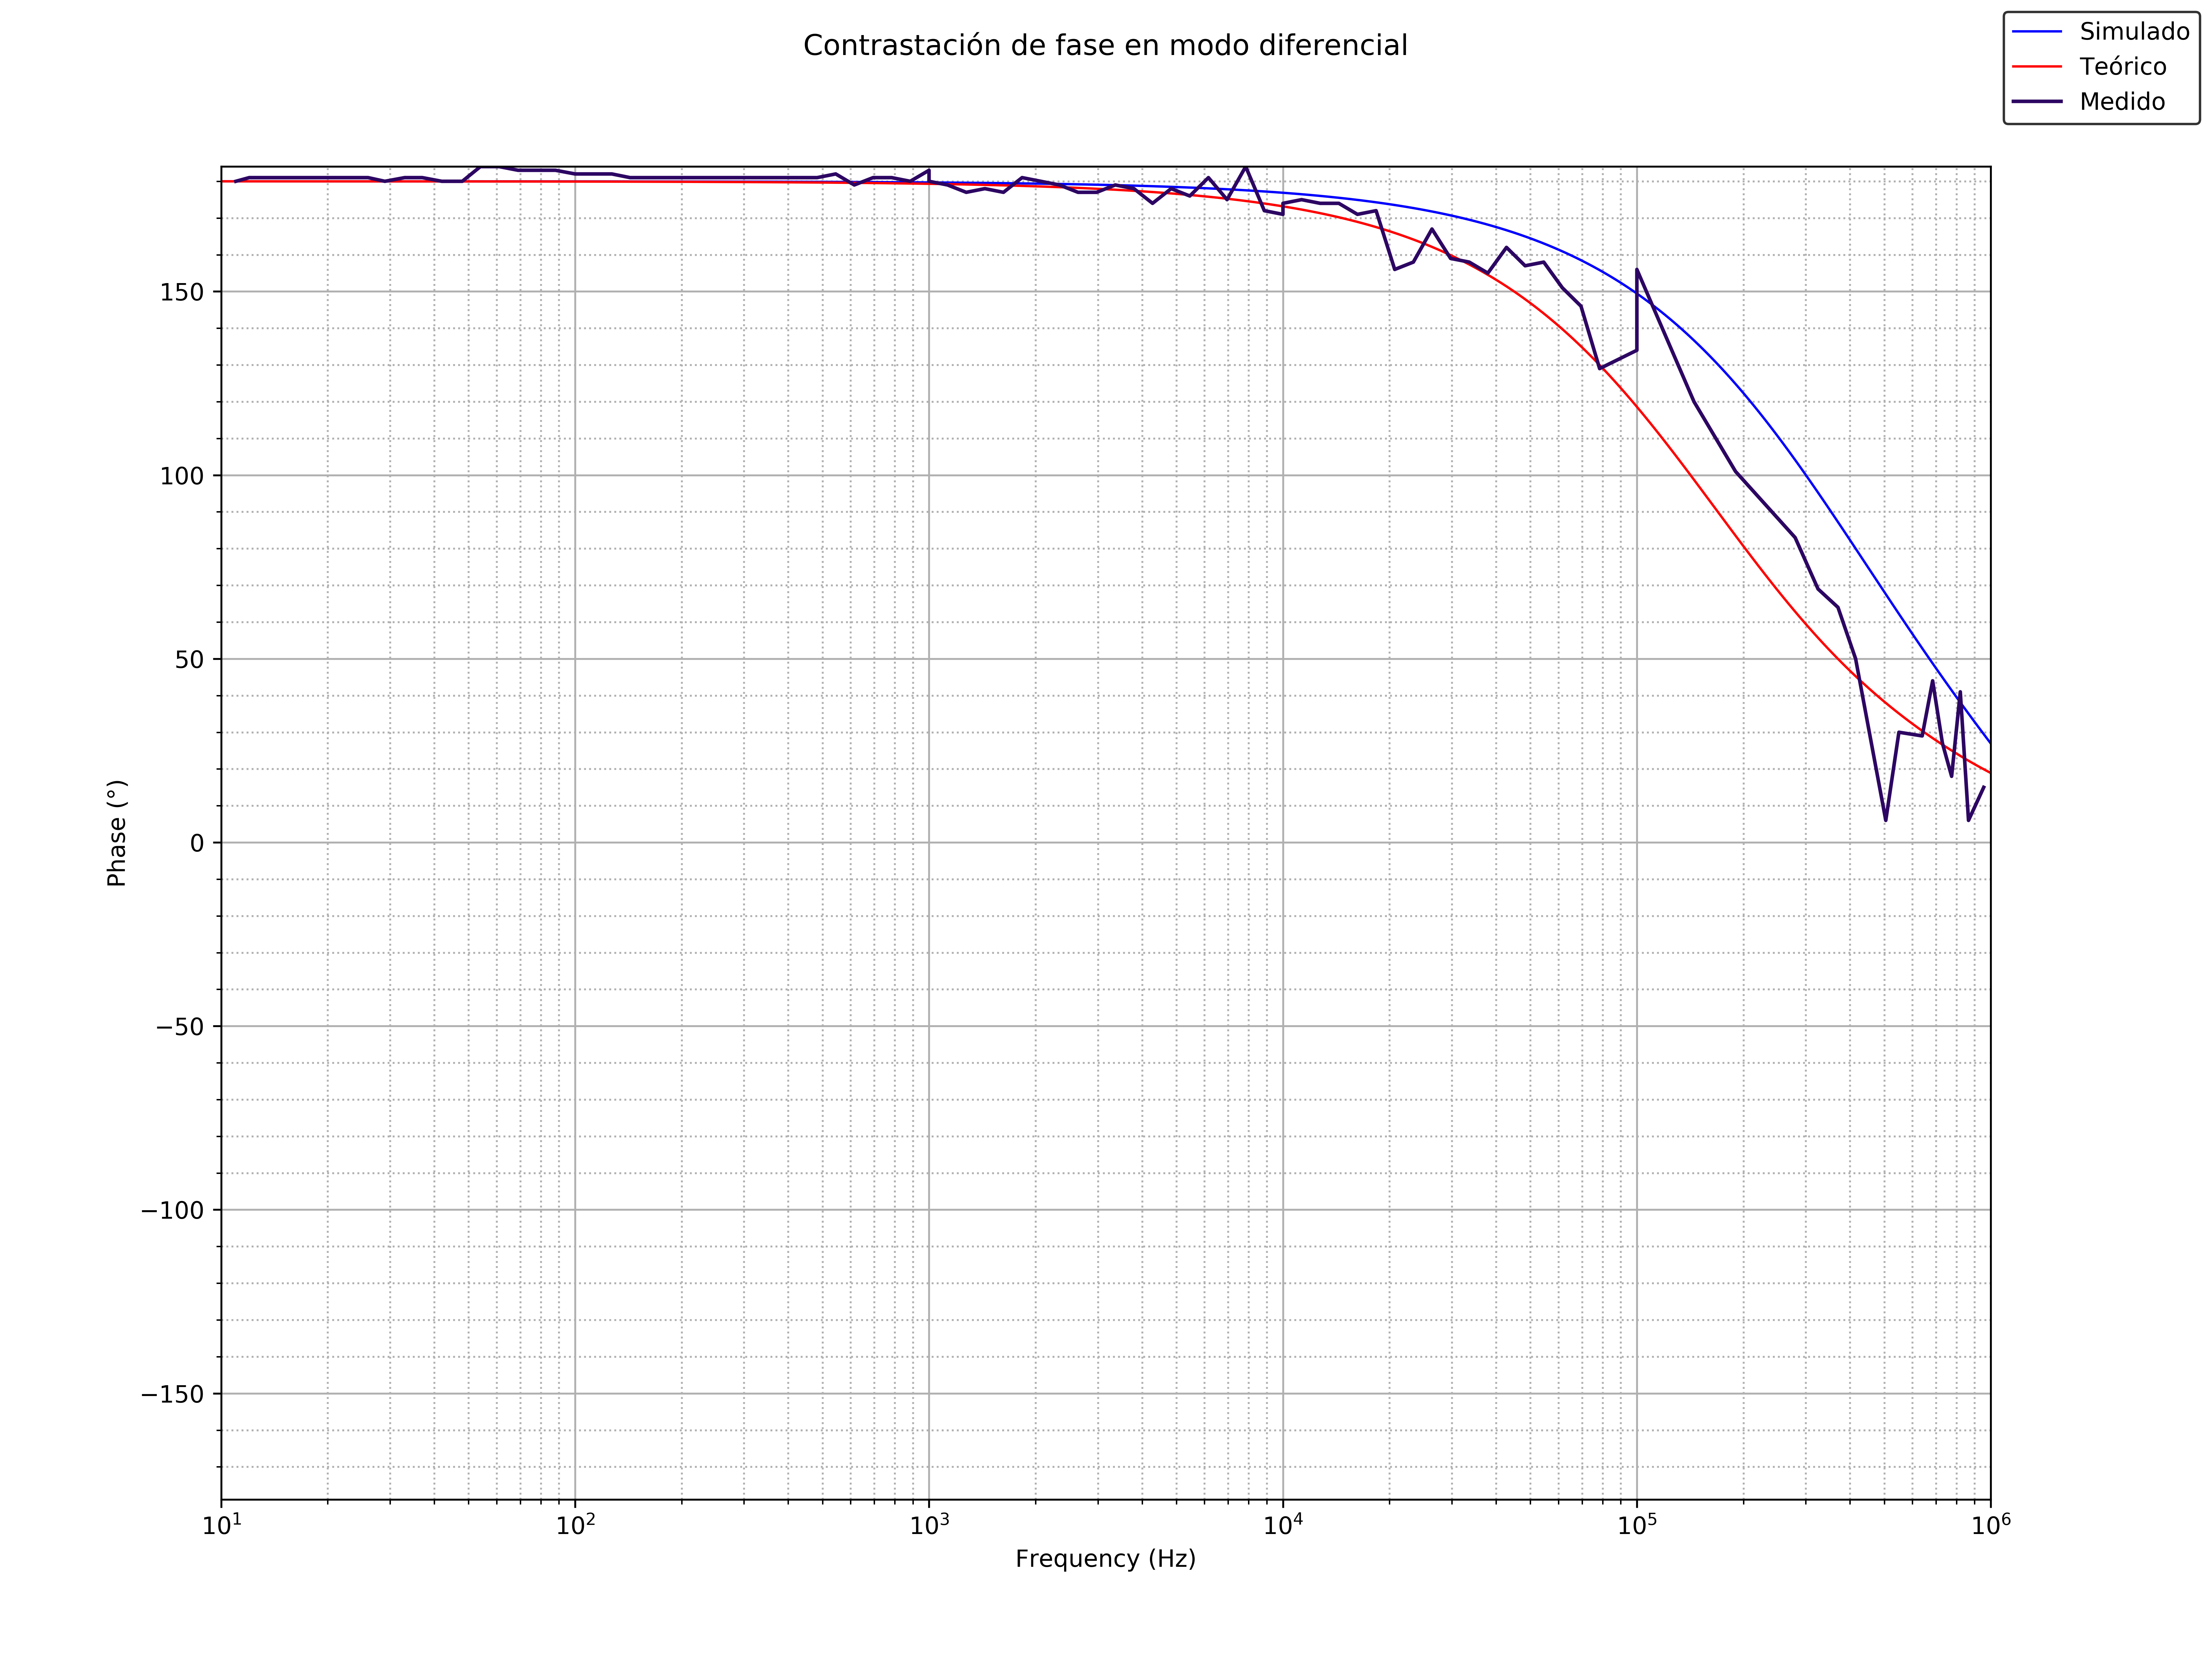
\includegraphics{../EJ3/Recursos/RES_PHA_DIF}

\end{tabular}%
}
\caption{Contrastaci\'on de modulo y fase medida, te\'orica y calculada para el circuito en modo diferencial}
\label{fig:RES_DIF}
\end{figure}


\begin{figure}[H]
    \centering
\resizebox{\textwidth}{!}{%
\begin{tabular}{c c}
    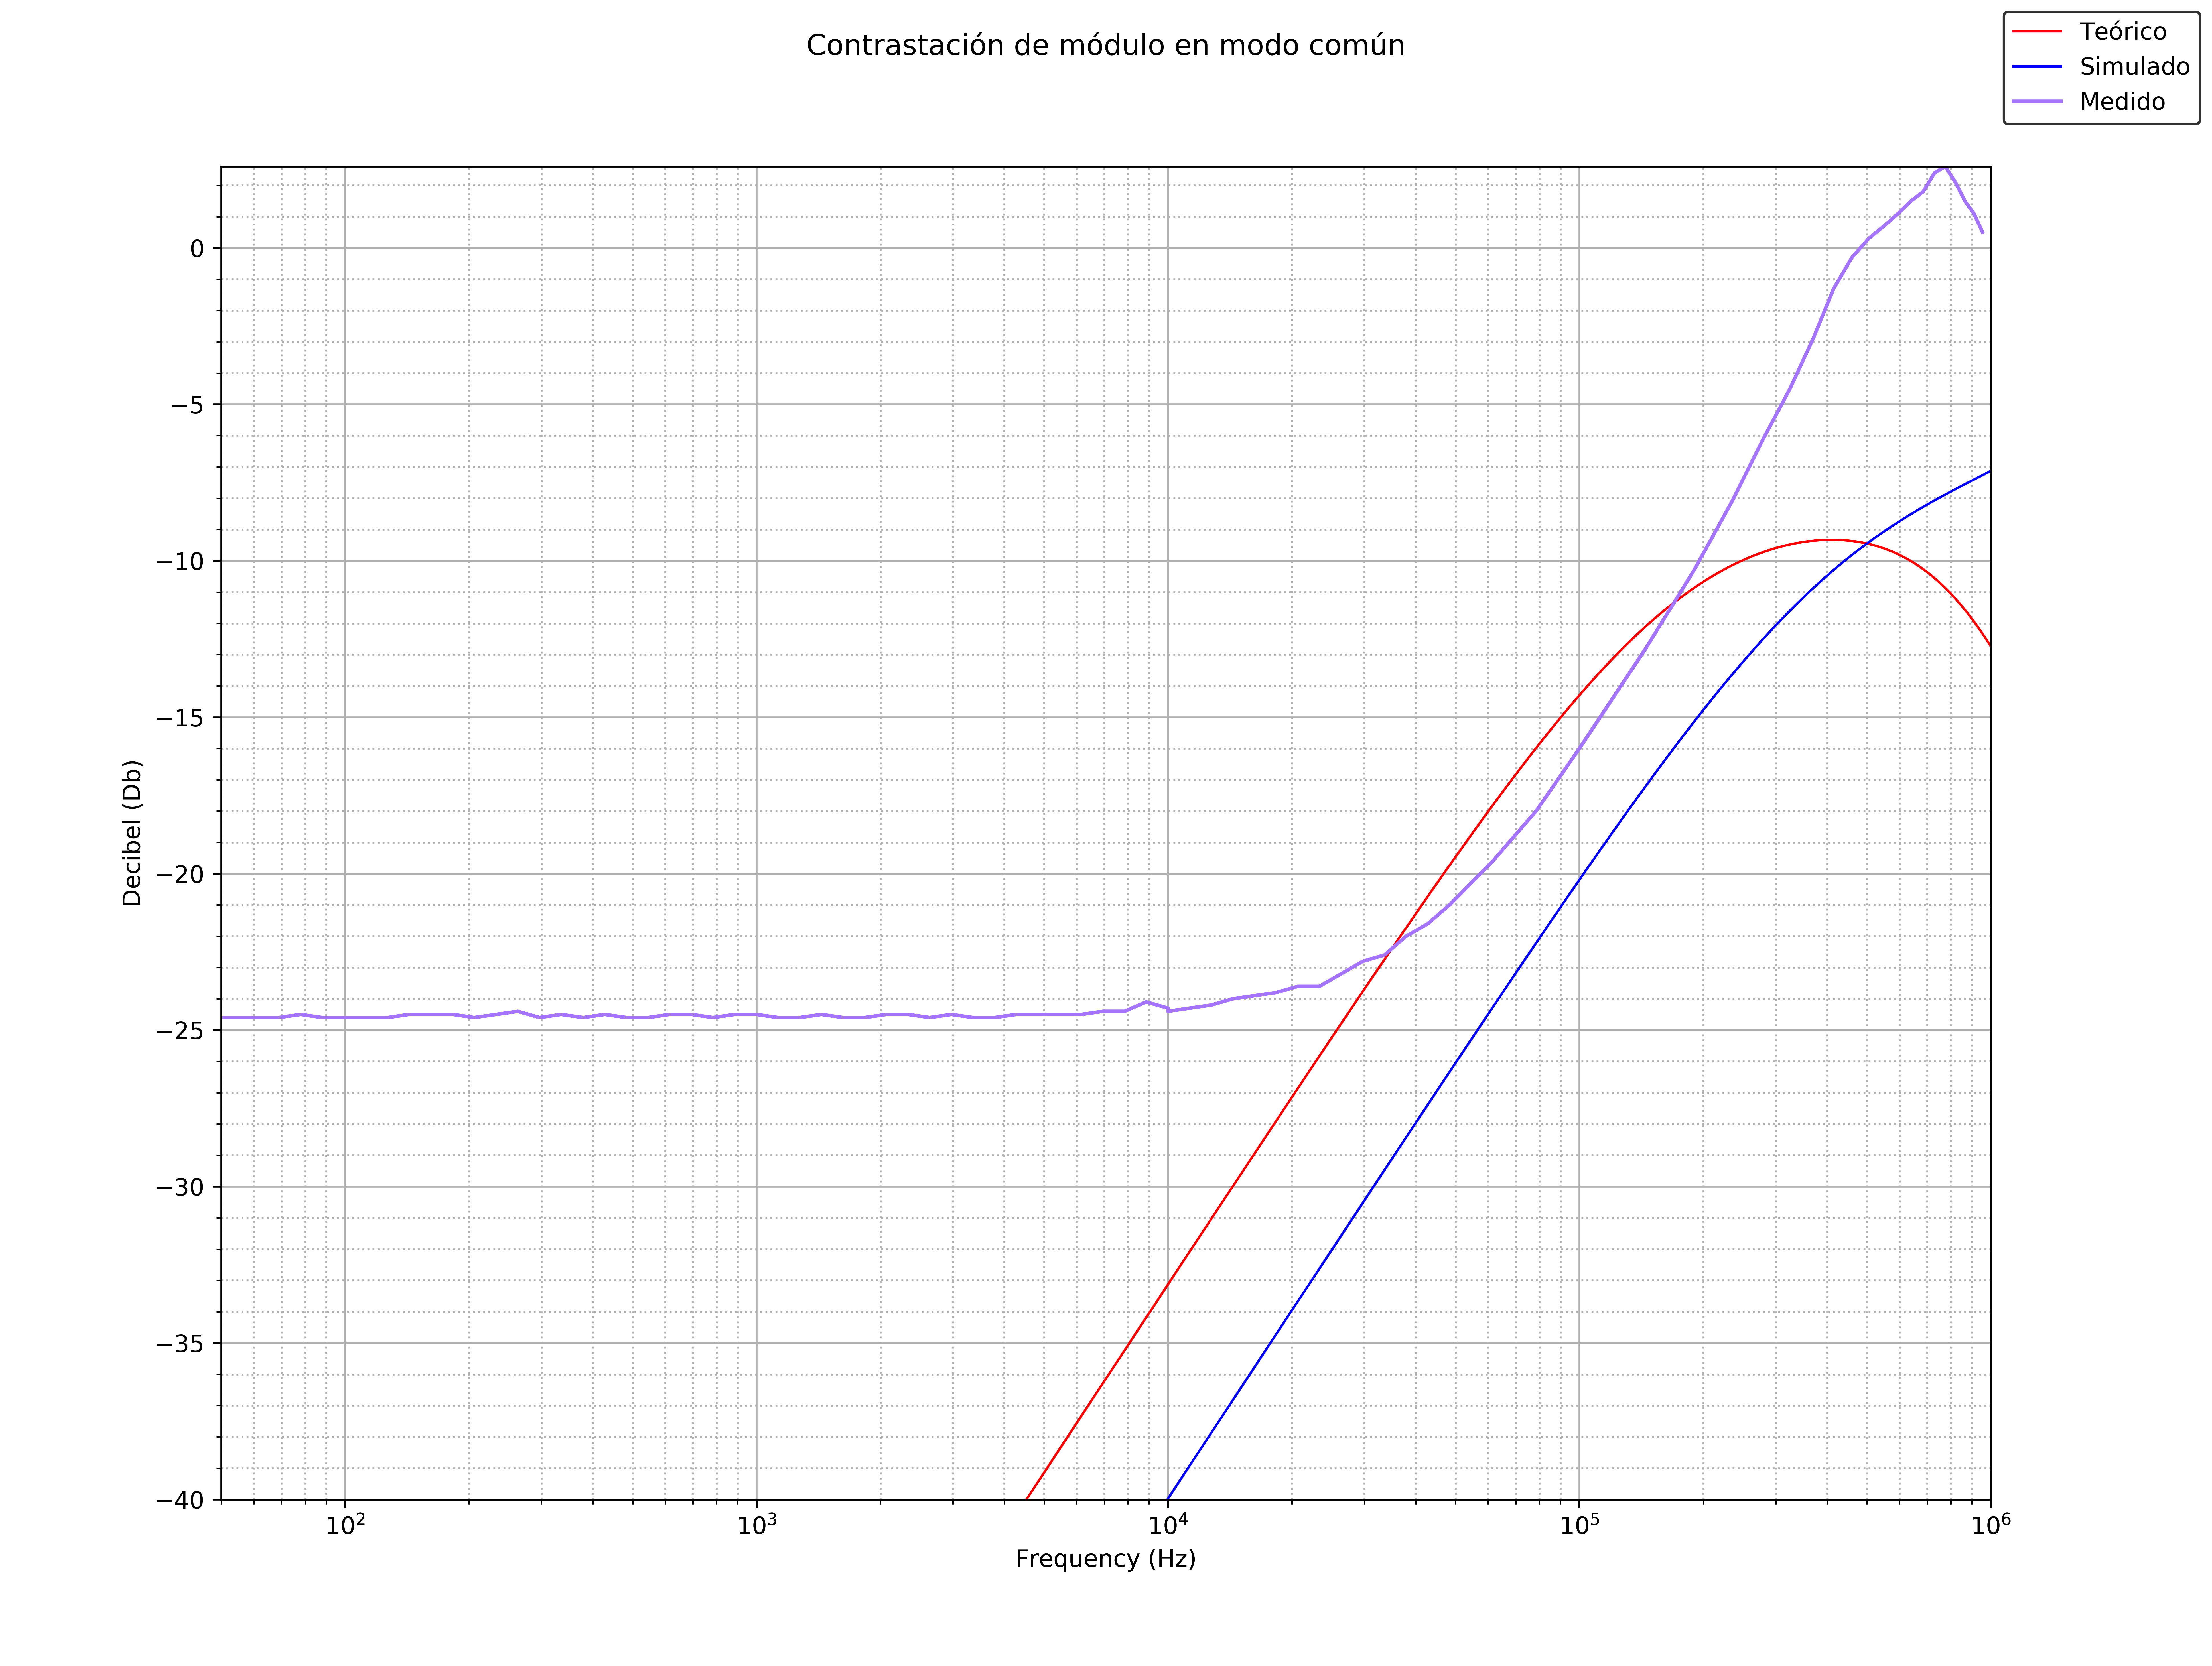
\includegraphics{../EJ3/Recursos/RES_MOD_COM} &
    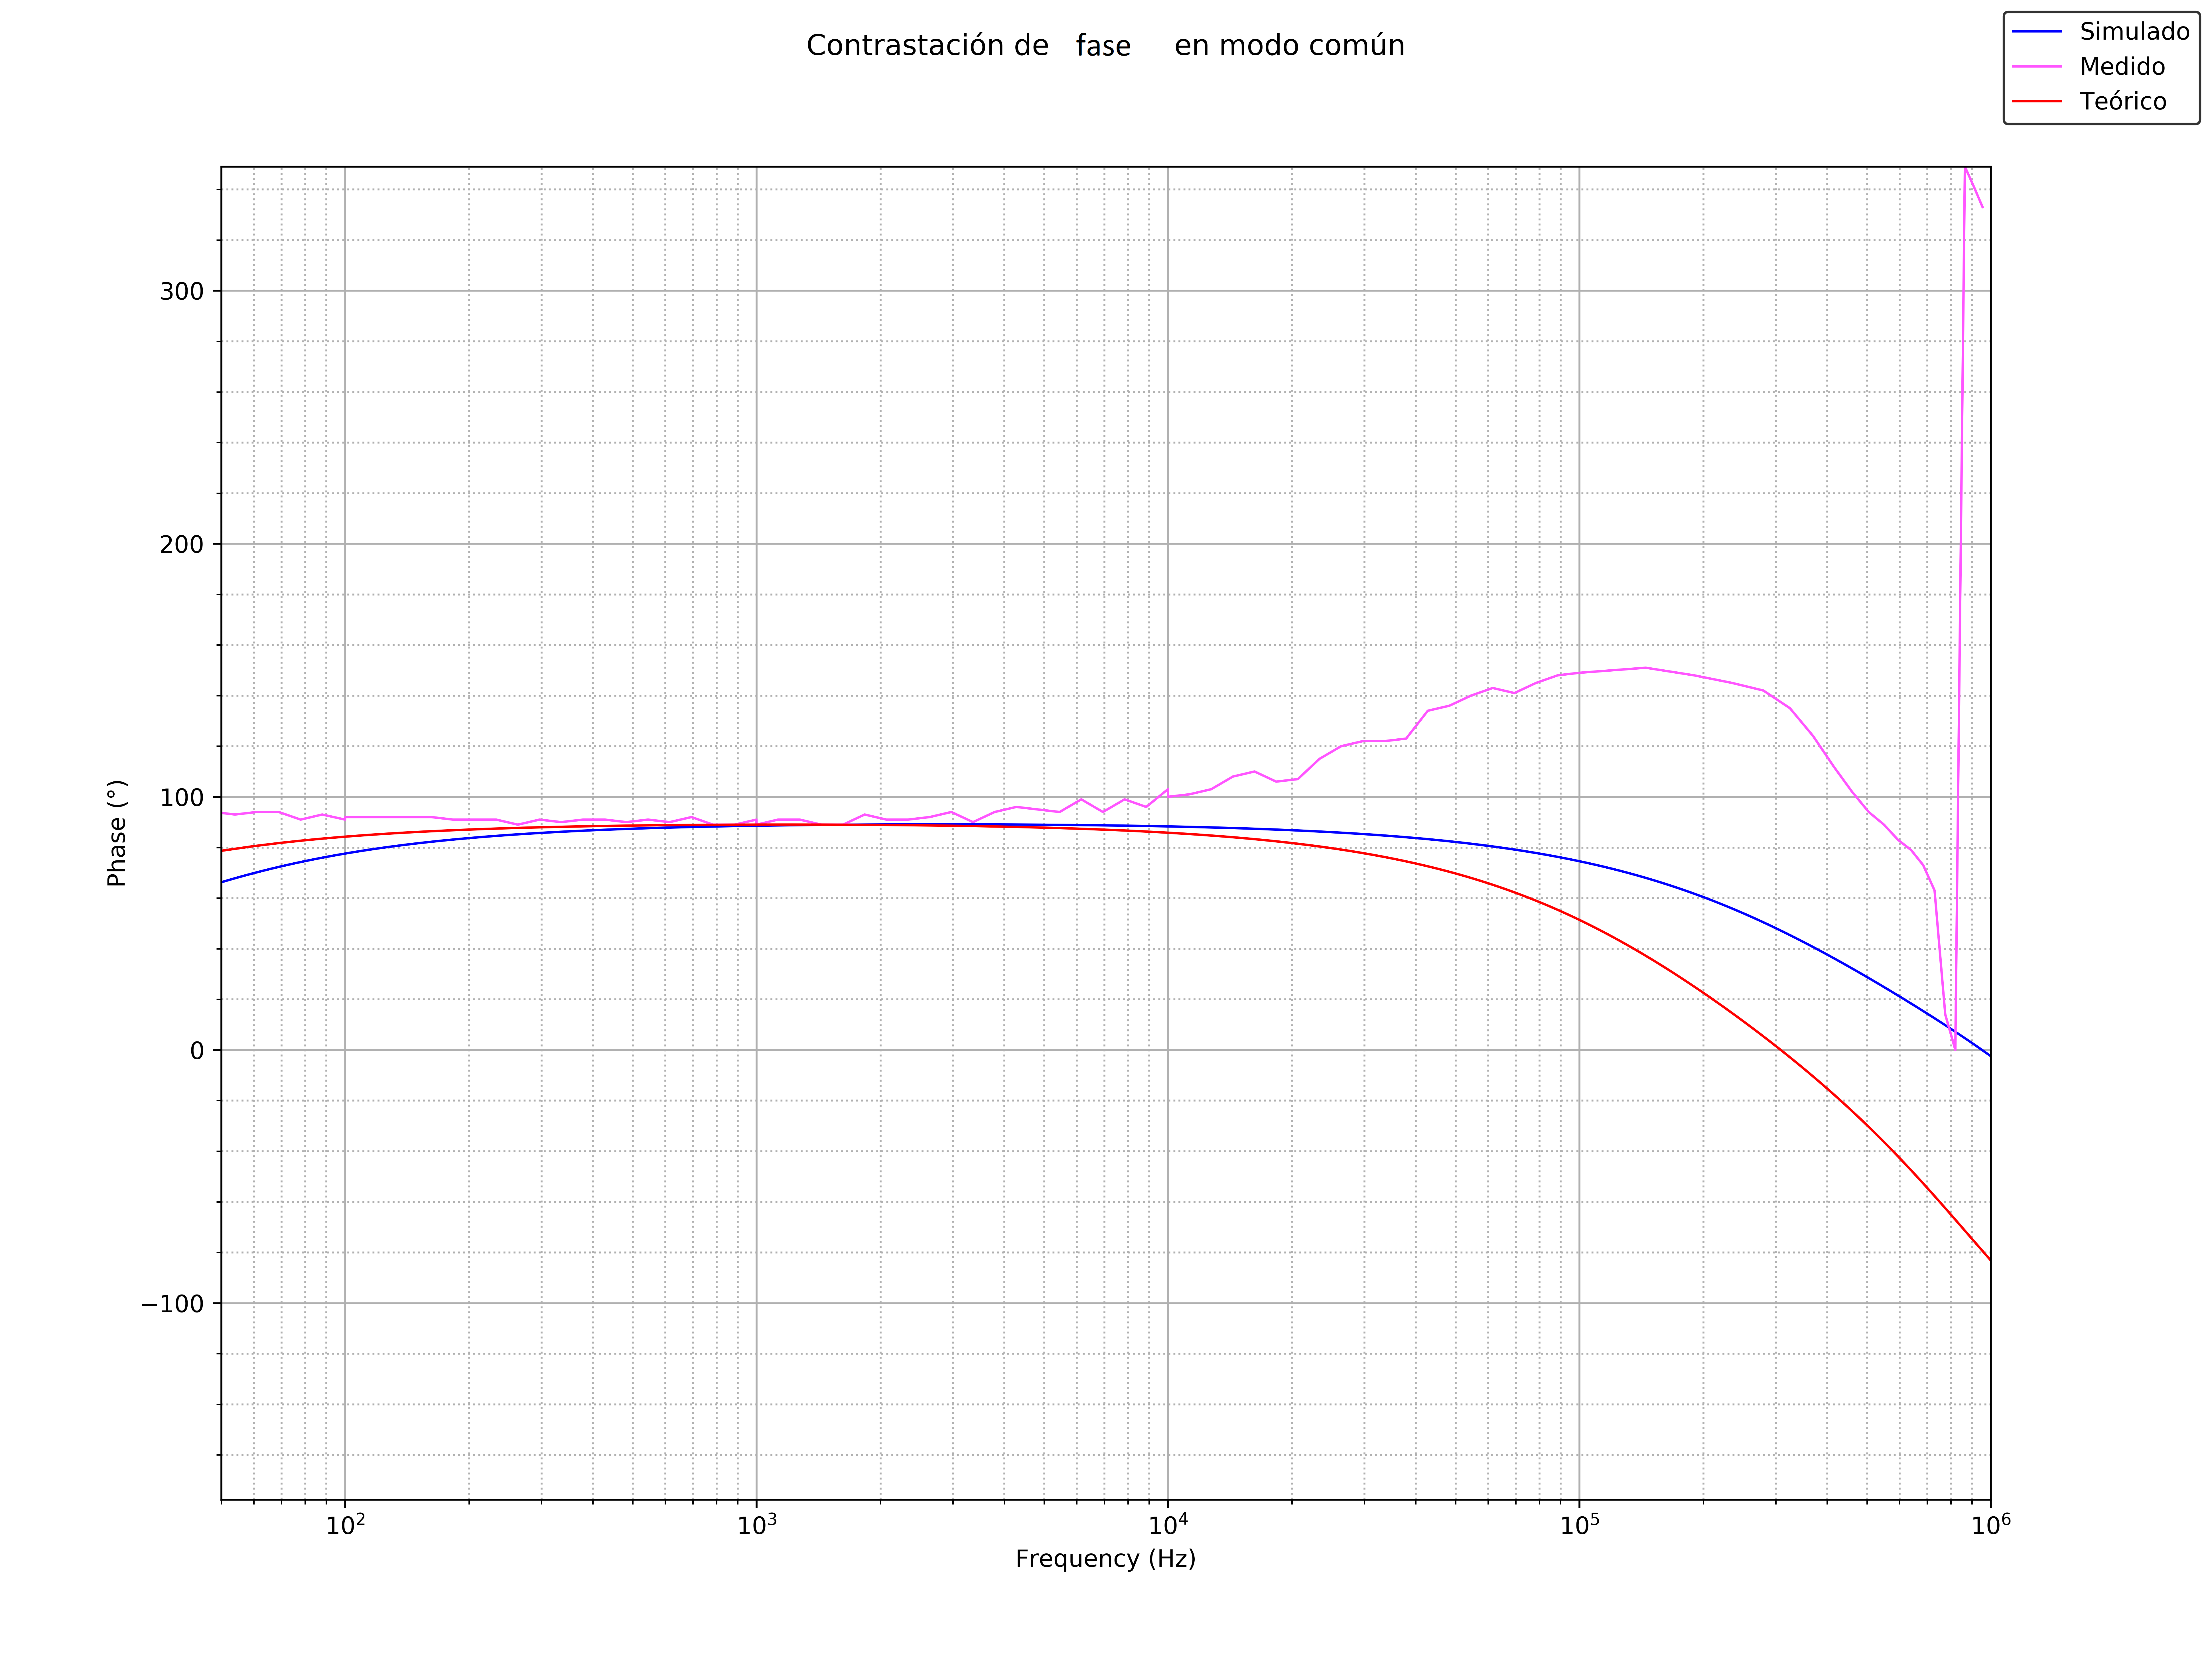
\includegraphics{../EJ3/Recursos/RES_PHA_COM}

\end{tabular}%
}
\caption{Contrastaci\'on de modulo y fase medida, te\'orica y calculada para el circuito en modo com\'un}
\label{fig:RES_COM}
\end{figure}
Se puede observar que los gr\'aficos cumplen con lo esperado. En modo diferencial se logra una gran similitud con lo medido y lo calculado, esto se relaciona directamente a la gran insensibilidad que presenta el amplificador de instrumentac\'on a las variaciones de sus componentes, cuando trabaja en modo diferencial. 
En cambio en el caso de modo com\'un se ve todo lo contrario, las curvas medidas no se ajustan tan bien como las anteriores. Sin embargo, este era un resultado esperado, ya que, para el modo com\'un el amplificador presenta una gran sensibilidad frente a peque\~nas variaciones en las tolerancias o los par\'ametros de los amplificadores operacionales. 
El \'unico gran defecto que presentan las mediciones con respecto a las simulaciones y el an\'alisis te\'orico, es que hay un rango de frecuencias cercanas a los 700KHz donde amplifica el modo com\'un. Este resultado no puede ser explicado a partir del an\'alisis te\'orico realizado ni a ninguna de las simulaciones. Se atribuye por lo tanto a una variable que no es tenida en cuenta ni siquiera por el modelo de LTSpice provisto y por lo tanto, resulta imposible de analizar.

\subsection{Puente de Wheatstone}
Se muestra en la Figura \ref{fig:puente} el puente de wheatstone. Mediante este es posible lograr un generador de se\~nales diferenciales 
que responde a la ecuaci\'on \ref{eq:puente}.
\begin{figure}[H]

    \centering
    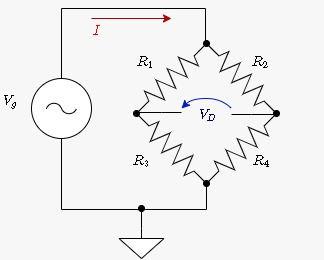
\includegraphics[width=0.5\textwidth]{../EJ3/Recursos/PUENTE}
    \caption{Salida del amplificador con entrada diferencial}
    \label{fig:puente}
\end{figure}
\begin{equation}
    V_D=\left(\frac{R_2 \cdot R_3 - R_1 \cdot R_4}{(R_1 + R_3)\cdot(R_2 + R_4))}\right)\cdot V_g
    \label{eq:puente}
\end{equation}
Donde $V_D$ es la amplitud de la se\~nal diferencial generada a la salida del puente y $V_g$ es la amplitud de la se\~nal de entrada del puente.

Por lo general, los puentes tienen una resistencia variable que permite lograr el equilibrio, lo que hace que la salida $V_D$ sea 0V. En este caso y con el fin de lograr un generador lo que fuera estable a lo largo del tiempo se decide utilizar la totalidad de las resistencias con un valor fijo.

Adem\'as como se sabe que la salida de este se conecta al amplificador, con una ganancia aproximada de 130 veces, se requiere de una se\~nal de baja amplitud que no provoque que sature el amplificador. Por lo tanto en puente debe estar cerca del equilibrio.

Teniendo todo esto en cuenta, se realiza el puente con 4 resistencias de valor nominal 10K y tolerancia del 5\%. Al medirlas se obtuvieron los valores que se muestran en \ref{eq:val_R}
\begin{equation}
    \begin{array}{llll}
    R1 = 9.87 K\Omega\\
    R2 = 9.81 K\Omega \\
    R3 = 9.94 K\Omega \\
    R4 = 9.99 K\Omega \\
    \end{array}
    \label{eq:val_R}
\end{equation}

Al reemplazar estos valores en \ref{eq:puente}, se obtiene una atenuaci\'on de aproximadamente 360 veces. Al alimentar el circuito con una tension de 7Vpp se debe obtener a la salida una se\~nal de 20mVpp, un valor dentro del rango que no hace saturar al amplificador. Esta se\~nal es amplificada 130 veces por el amplificador, con lo que se obtiene, a la salida la se\~nal que se observa en la Figura \ref{fig:inDIF}.
\begin{figure}[H]

    \centering
    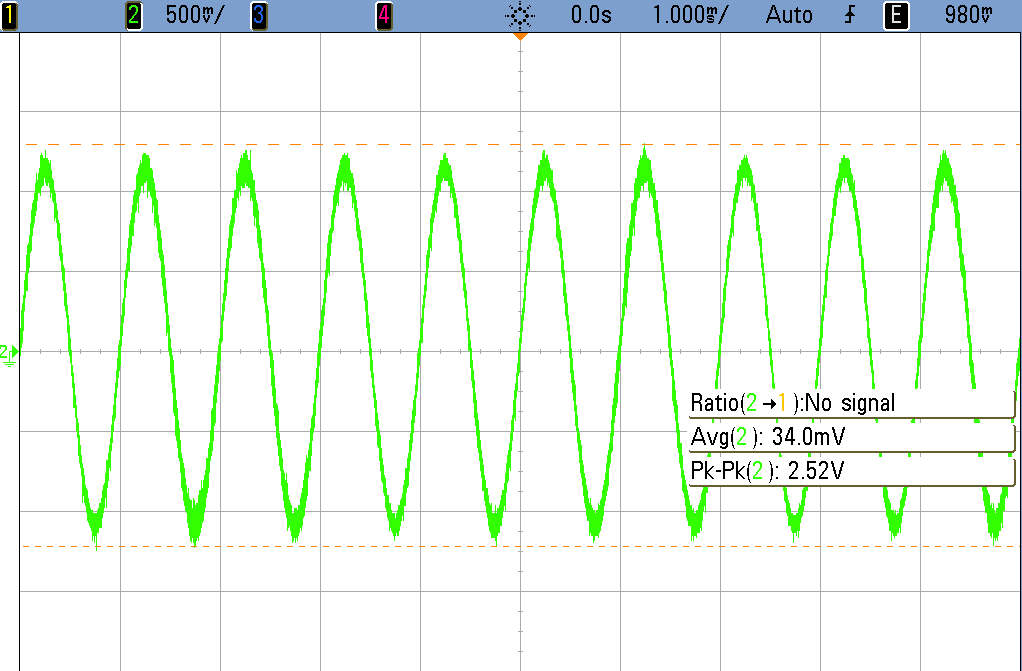
\includegraphics[width=0.5\textwidth]{../EJ3/Recursos/Salida_inDIF}
    \caption{Salida del amplificador con entrada diferencial}
    \label{fig:inDIF}
\end{figure}
 
Se obtiene una salida de 2.5Vpp, lo que se corresponde con lo esperado. Adem\'as es importante se\~nalar que, el ruido observado a la salida del amplificador es mucho menor que es que se observa en la se\~nal de entrada. No se presenta una imagen representativa de esta ya que, cuando se realiz\'o la medici\'on, de esta secci\'on no se conect\'o correctamente el osciloscopio para medir la salida diferencial, lo que lleva a una se\~nal que no se corresponde con la entrada real, por lo que se decide no agregarla.


\subsection{DC offset}
\subsubsection{An\'alsis te\'orico}
Se propone, con la finalidad de montar la salida en una tensi\'on continua de offset, el circuito de la Figura \ref{fig:AMP_INST_OFFSET}
\begin{figure}[H]

    \centering
    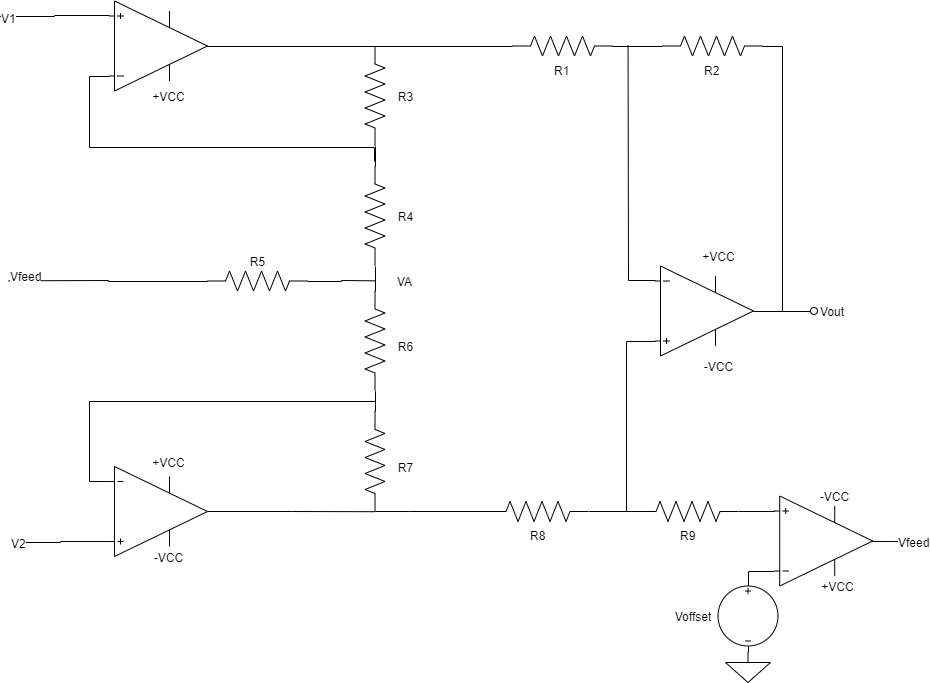
\includegraphics[width=0.5\textwidth]{../EJ3/Recursos/AMP_INST_OFFSET}
    \caption{Circuito propuesto para agregar una $V_{offset}$ de continua a la salida}
    \label{fig:AMP_INST_OFFSET}
\end{figure}
Para hacer el an\'alisis en esta secci\'on se recurre al sistema de ecuaciones \ref{eq:sist_ideal}.
Observando las ecuaciones se puede observar que, debido a la masa virtual en el borne no inversor del operacional 4 se obtiene que $V_{o2} = V_{offset}$.
Si se realiza nuevamente el an\'alisis del circuito, pero en este caso con la condici\'on para modo com\'un $V_1 = V_2 \implies V_{out} = V_{offset}$. Se llega, entonces, a \ref{eq:soluc_conDC} donde se puede ver claramente como afecta el offset a la salida.
\begin{equation}
    V_{out} = V_{offset}-\frac{R_2}{R_1} \cdot \left(1+\frac{R_3}{R_4}\right)\cdot \left(V_1-V_2\right)
    \label{eq:soluc_conDC}
\end{equation}
\subsubsection{Constrastaci\'on pr\'actica}
Se puede observar en la Figura \ref{fig:VDC_BIEN} los resultados obtenidos al inyectar una continua de $V_{offset}=5V$

\begin{figure}[H]

    \centering
    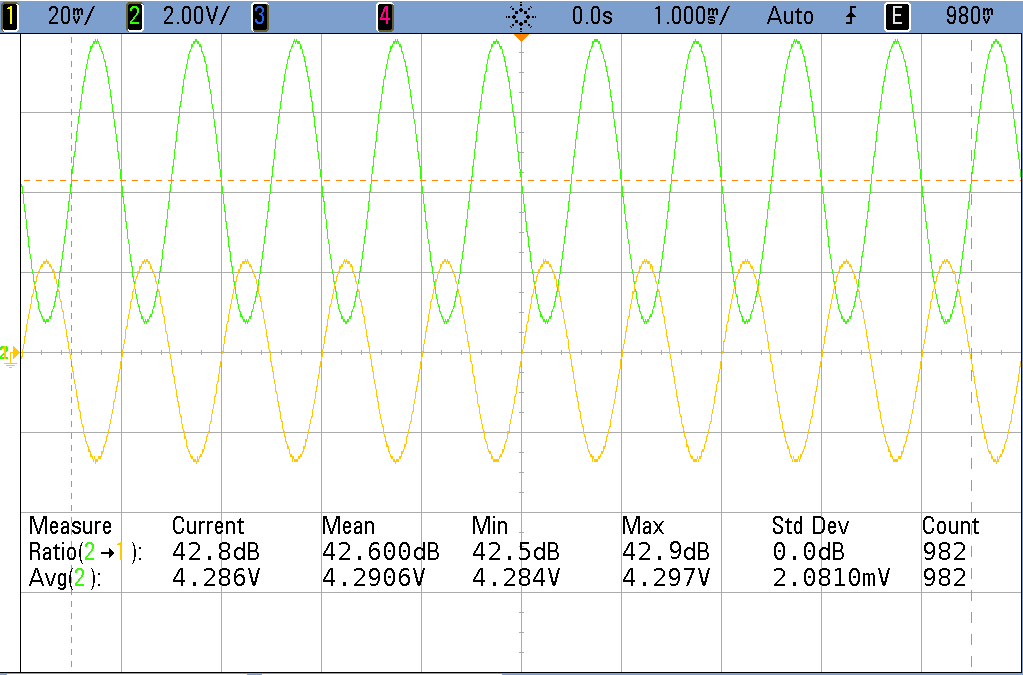
\includegraphics[width=0.5\textwidth]{../EJ3/Recursos/DC_5V}
    \caption{Salida montada sobre una continua con $R_5 = 30 K\Omega$}
    \label{fig:VDC_BIEN}
\end{figure}


El resultado es el esperado, la se\~nal se encuentra montada sobre una tensi\'on continua cercana a los 5V.

\subsubsection{Diferencias con la teor\'ia}
Se muestra en la Figura \ref{fig:VDC_MAL} la diferencia encontrada respecto de la teor\'ia

\begin{figure}[H]

    \centering
    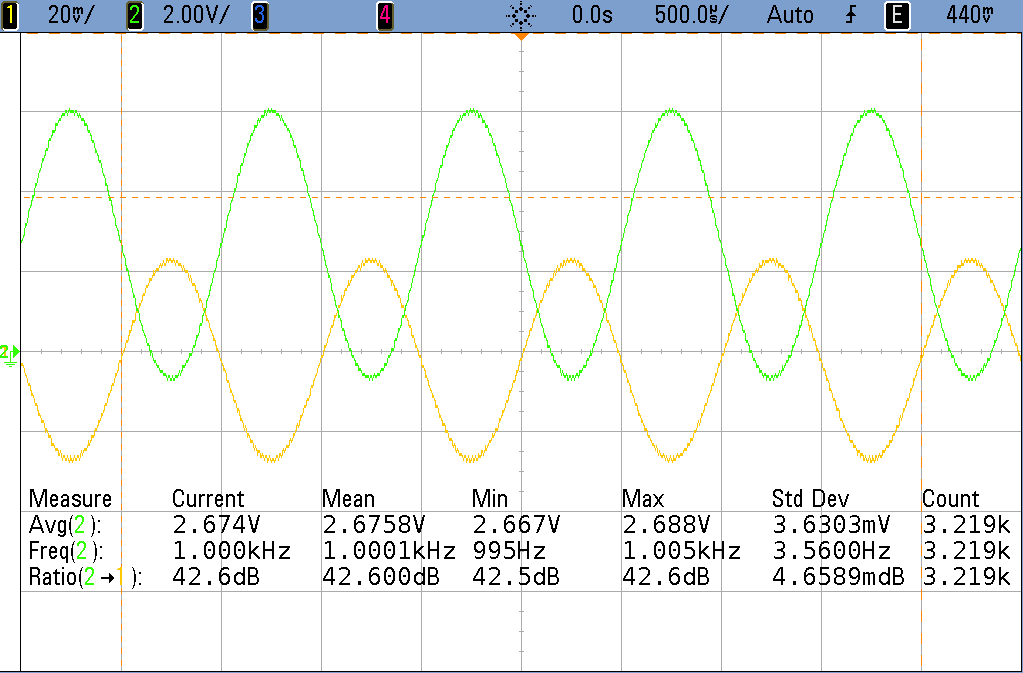
\includegraphics[width=0.5\textwidth]{../EJ3/Recursos/DC_27}
    \caption{Salida montada sobre una continua con $R_5 = 50 K\Omega$}
    \label{fig:VDC_MAL}
\end{figure}


Se puede observar que a pesar de los resultados obtenidos a partir de los c\'alculos, la se\~al esta montada sobre un nivel de continua menor a 5V, cercano a los 3V. Esto es debido a que se encuentra, en base al valor de $R_5$, una variac\'on en el valor de tensi\'on al que se monta la se\~nal. Para este caso, se realiza la medici\'on con un valor de $R_5 = 50 K\Omega$ 
Esta relaci\'on no puede explicarse en base al an\'alisis ideal, sin embargo, es posible observar en las simulaciones con todos los operacionales reales, que efectivamente esto es lo que se obtiene.




\subsection{Mediciones sin referencia a tierra}
Es importante que el amplificador de instrumentaci\'on este referido a la misma conexi\'on a tierra que su entrada. Esta importancia se pone de manifiesto en \ref{eq:soluc_conDC}, pues lo que sea que se conecte a la entrada inversora del operacional 4, aparece a la salida sumado a la se\~nal.
Esto afecta directamente al amplificador, debido a que si las tierras no son compartidas, es posible que se encuentren a un potencial distinto. Esta diferencia de potencial, de la que el ruido forma parte, se ver\'a a la salida del amplificador casi sin ninguna atenuaci\'on, lo que va en contra de la caracter\'istica principal del amplificador de instrumentaci\'on que es su gran CMRR. 

Sin embargo, al realizar las mediciones pertinentes con las tierras aisladas la diferencia observada es muy peque\~na.
Esto se atribuye a la falla en el dise\~no del amplificador, que al no atenuar el ruido en todo el rango de frecuencias, no permite observar las peque\~nas variaciones debidas al ruido intruducido por la separaci\'on del las tierras.
Se muestran en la Figura \ref{fig:GND_notConnected} las mediciones obtenidas a 1KHz con las masas sin referenciar.

\begin{figure}[H]
    \centering
\resizebox{\textwidth}{!}{%
\begin{tabular}{c c}
    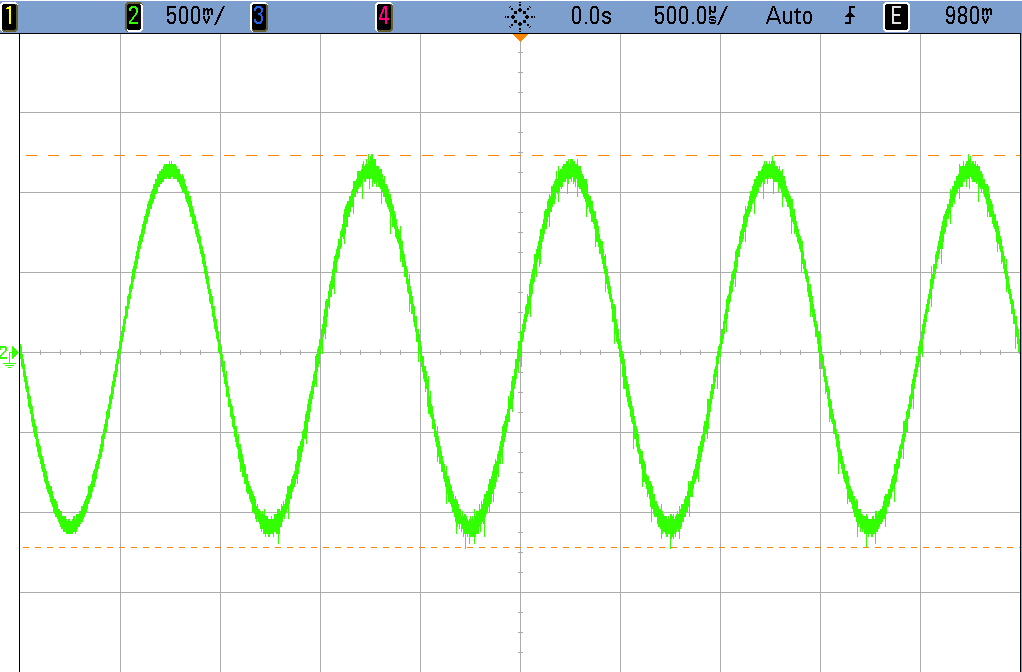
\includegraphics{../EJ3/Recursos/ref} &
    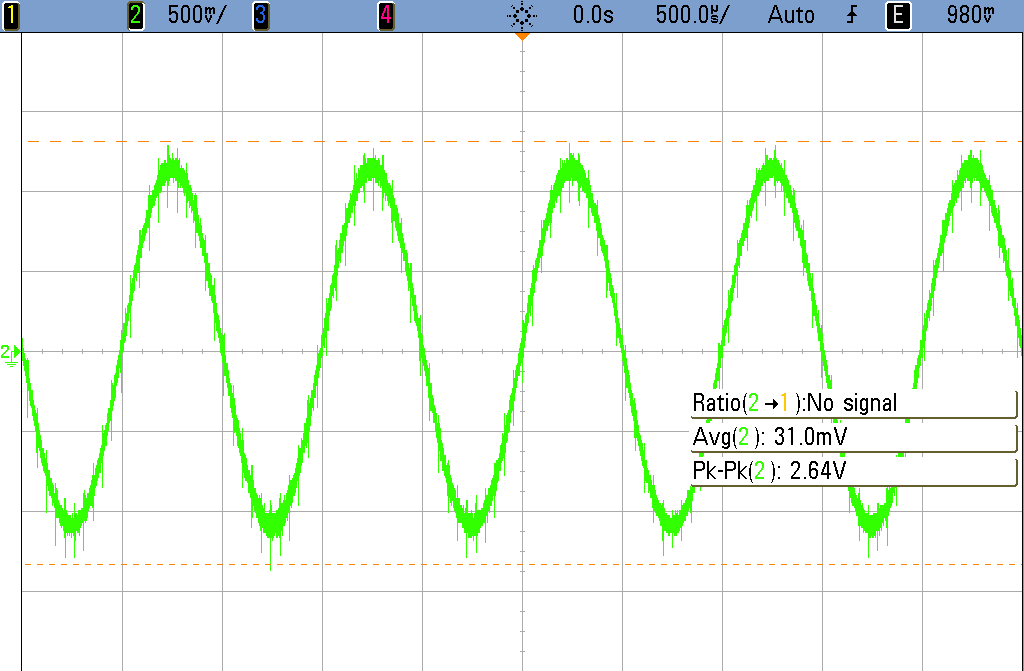
\includegraphics{../EJ3/Recursos/No_ref}

\end{tabular}%
}
\caption{Salida del amplificador, con(izquierda) y sin (derecha) masas referenciadas}
\label{fig:GND_notConnected}
\end{figure}
